\chapter{Preliminaries}\label{ch-0}
%\pagenumbering{arabic} % use this only if we revert to roman numerals for the front matter

This chapter reviews some of the basic concepts used in this text. Many can be
found in standard texts on discrete mathematics. Much of the notation employed
in later chapters is also presented here.

\section{Logic and Set Theory}\label{sec-0.1}
A basic familiarity with the nature of formal proofs is assumed; most proofs
given in this text are complete and rigorous, and the reader is encouraged to
work the exercises in similar detail. A knowledge of logic circuits would be
necessary to construct the machines discussed in this text. Important
terminology and techniques are reviewed here.

Unambiguous \emph{statements} that can take on the values {\bf True} or {\bf False} 
(denoted by $1$ and $0$, respectively) can be combined with \emph{connectives} such as
{\em and} ($\wedge$), {\em or} ($\vee$), and {\em not} ($\neg$)
to form more complex statements.
The truth tables for several useful connectives are given in Figure \ref{fig-0.1},
along with the symbols representing the physical devices that implement these
connectives.

As an example of a complex statement, consider the assertion that two statements
$p$ and $q$ take on the same value. This can be rephrased as:
Either ($p$ is true and $q$ is true) or ($p$ is false and $q$ is false).  As the
truth table for {\em not} shows, a statement r is false exactly when $\neg$r is
true; the above assertion could be further refined to:
Either ($p$ is true and $q$ is true) or ($\neg p$ is true and $\neg q$ is true).

% Figure 0.1
\begin{figure}
\begin{center} 
% top of fig0.1 same as fig1.14:
\centerline{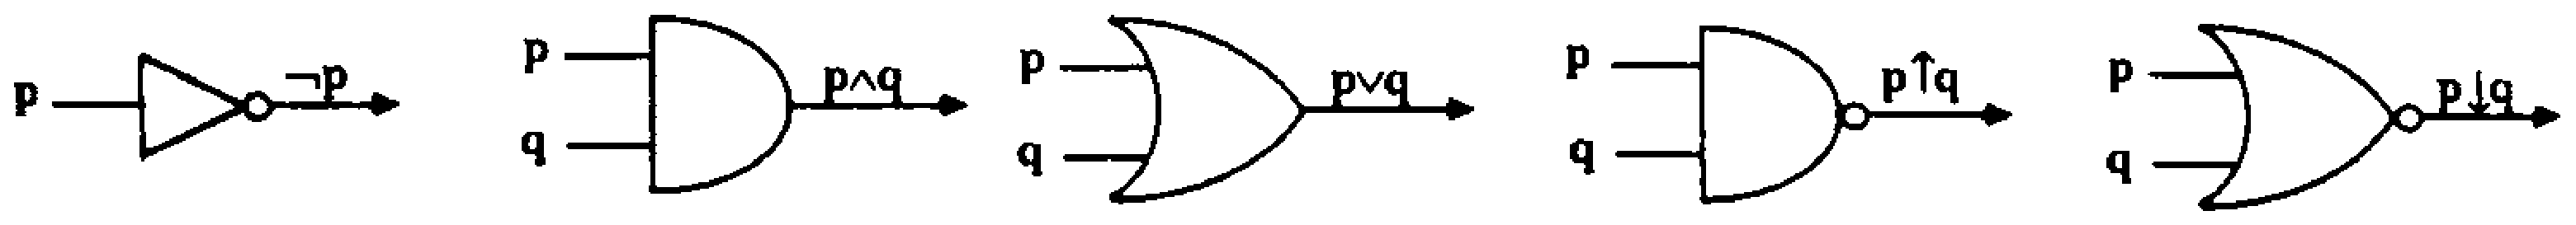
\epsfig{figure=ToFAfigures/fig1-14.eps,width=5.7in}}
\begin{tabular}{ccccc} 
%\fbox{IMAGE} & \fbox{IMAGE} & \fbox{IMAGE} & \fbox{IMAGE} & \fbox{IMAGE} \\ 
NOT gate & AND gate & OR gate & NAND gate & NOR gate \\ 
{ 
\begin{tabular}[b]{c|c} 
$p$ & $\neg p$ \\ 
\hline 
1 & 0 \\ 
0 & 1 
\end{tabular} 
} & { 
\begin{tabular}{cc|c} 
$p$ & $q$ & $p\wedge q$ \\ 
\hline 
1 & 1 & 1 \\ 
1 & 0 & 0 \\ 
0 & 1 & 0 \\ 
0 & 0 & 0 
\end{tabular} 
} & { 
\begin{tabular}{cc|c} 
$p$ & $q$ & $p\vee q$ \\ 
\hline 
1 & 1 & 1 \\ 
1 & 0 & 1 \\ 
0 & 1 & 1 \\ 
0 & 0 & 0 
\end{tabular}
} & { 
\begin{tabular}{cc|c} 
$p$ & $q$ & $p \uparrow q$ \\ 
\hline 
1 & 1 & 0 \\ 
1 & 0 & 1 \\ 
0 & 1 & 1 \\ 
0 & 0 & 1 
\end{tabular} 
} & { 
\begin{tabular}{cc|c} 
$p$ & $q$ & $p \downarrow q$ \\ 
\hline 
1 & 1 & 0 \\ 
1 & 0 & 0 \\ 
0 & 1 & 0 \\ 
0 & 0 & 1 
\end{tabular} 
} 
\end{tabular} 
\end{center}
\caption{Common logic gates and their truth tables}\label{fig-0.1}
\end{figure}


In symbols, this can be abbreviated as:
$$(p \wedge q) \vee (\neg p \wedge \neg q)$$
The truth table covering the four combinations of truth values of $p$ and $q$
can be built from the truth tables defining $\wedge$, $\vee$, and $\neg$, as
shown in \ref{fig-0.2}. The truth table shows that the assertion is indeed
true in the two cases where $p$ and $q$ reflect the same values, and false in
the two cases where the values assigned to $p$ and $q$ differ. When the statement
that $r$ and $s$ always take on the same value is indeed true, we often write
$r$\ {\em iff}\ $s$ (``$r$ if and only if $s$''). The \Index{biconditional} can also be denoted by
$r \Leftrightarrow s$ (``$r$ is \emph{equivalent} to $s$'').\index{equivalent!logical expressions}

% Figure 0.2
\begin{figure}[tb]
\begin{center}
\begin{tabular}{cc|ccccc}
$p$ & $q$ & $\neg p$ & $\neg q$ & $\neg p\wedge\neg q$ & $p\wedge q$ &
	$(p\wedge q)\vee(\neg p\wedge\neg q)$\\
\hline
1 & 1 & 0 & 0 & 0 & 1 & 1\\
1 & 0 & 0 & 1 & 0 & 0 & 0\\
0 & 1 & 1 & 0 & 0 & 0 & 0\\
0 & 0 & 1 & 1 & 1 & 0 & 1
\end{tabular}
\end{center}
\caption{Truth tables for various compound expressions}\label{fig-0.2}
\end{figure}

Consider the statement $(p \wedge q) \vee (p \downarrow q)$.
Truth tables can be constructed to
verify that $(p \wedge q)  \vee (\neg p \wedge \neg q)$ and 
$(p \wedge q) \vee (p \downarrow q)$ have identical truth tables, and
thus $(p \wedge q) \vee (\neg p \wedge \neg q) \Leftrightarrow (p \wedge q)
\vee (p \downarrow q)$.

\subsection*{Example 0.1}

Circuitry for realizing each of the above statements is displayed in Figure
\ref{fig-0.3}. Since the two statements were equivalent, the circuits will
exhibit the same behavior for all combinations of input signals $p$ and $q$.
The second circuit would be less costly to build since it contains fewer
components, and tangible benefits therefore arise when equivalent but less
cumbersome statements can be derived. Techniques for \emph{minimizing} such circuitry
are presented in most discrete mathematics texts.

Example 0.1 shows that it is straightforward to implement statement formulas
by circuitry. Recall that the location of the $1$ values in the truth table can
be used to find the corresponding \emph{\Index{principal disjunctive normal
form}} (\Index{PDNF}) for the expression represented by the truth table. For
example, the truth table corresponding to NAND has three rows with $1$ values
$(p = 1, q = 0; p = 0, q = 1; p = 0, q = 0)$, leading to three \emph{terms} in the PDNF
expression: $(p \wedge \neg q) \vee (\neg p \wedge q) \vee  (\neg p \wedge \neg
q)$. This formula can be implemented as the circuit illustrated in Figure
\ref{fig-0.4} and thus a NAND gate can be replaced by this combination of three
ANDs and one OR gate. This circuit relies on the assurance that a quantity of
interest (such as $p$) will generally be available in both its negated and
unnegated forms. Hence we can count on access to an input line representing
$\neg p$ (rather than feeding the input for $p$ into a NOT gate).

% Figure 0.3
\begin{figure}[tb]
%\centerline{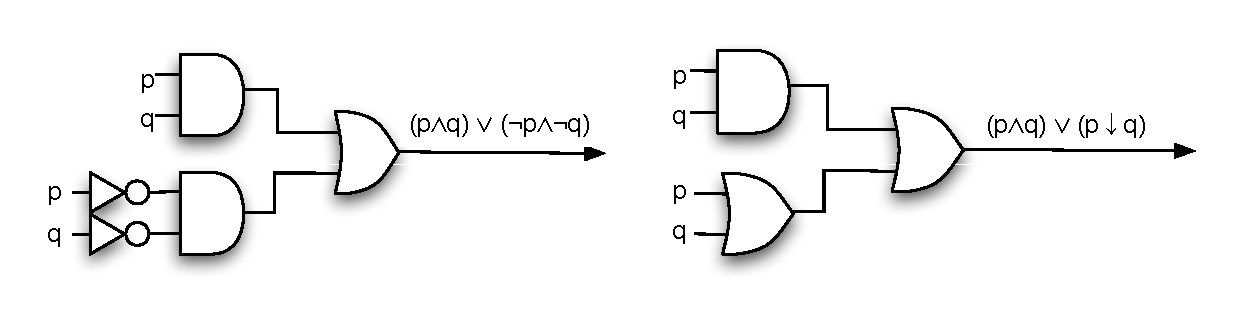
\epsfig{figure=Figures/fig-0-3.eps,width=\textwidth}}
\centerline{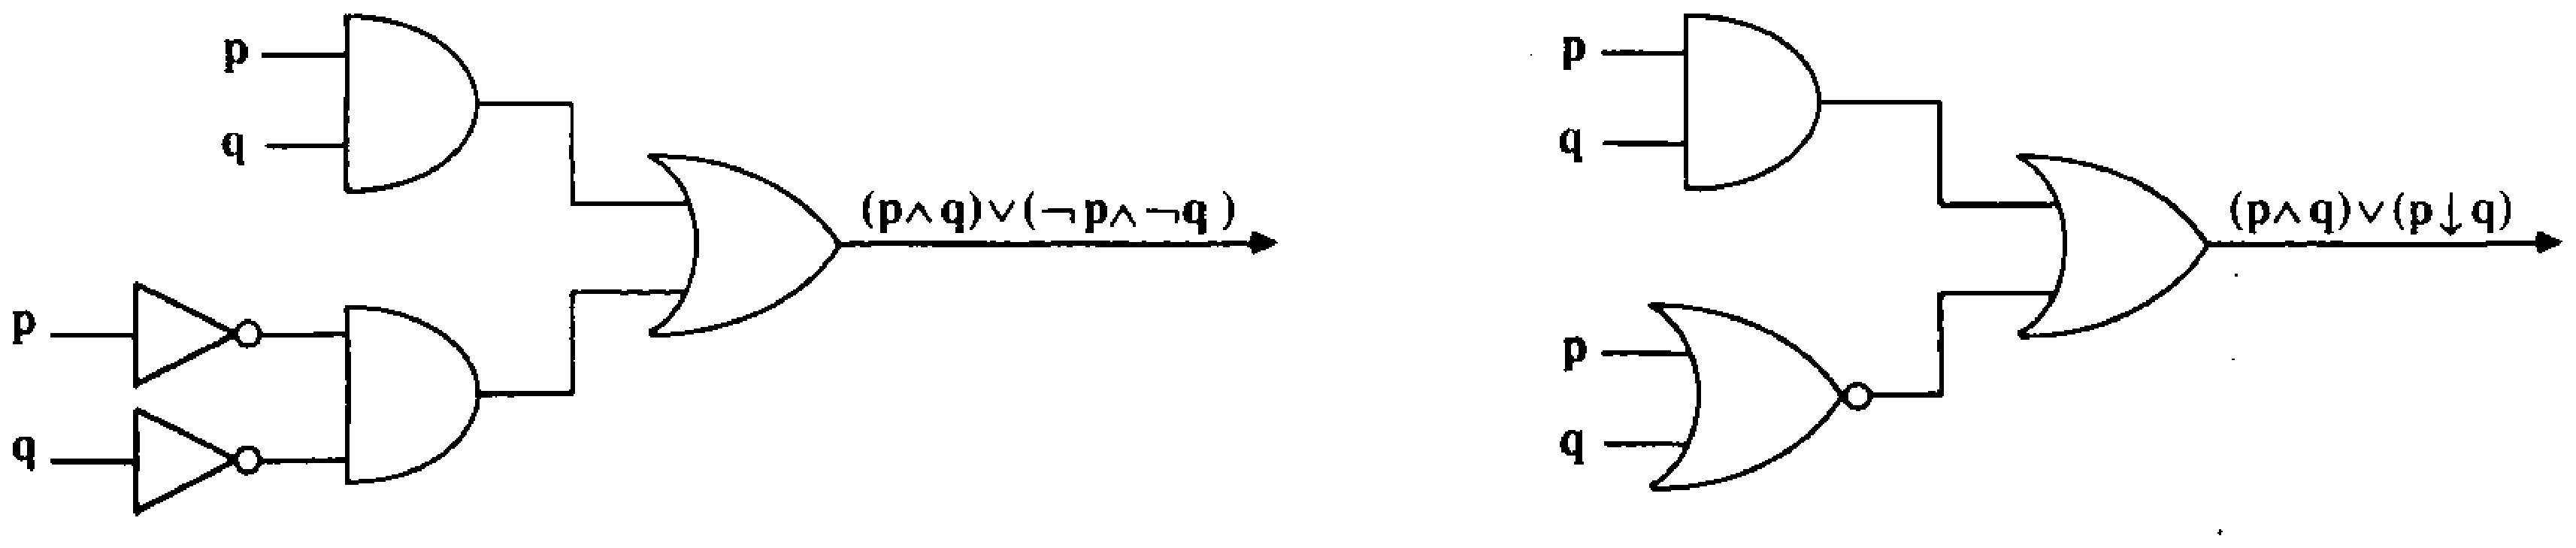
\epsfig{figure=ToFAfigures/fig0-3.eps,width=6.5in}}
\caption{Functionally equivalent circuits}\label{fig-0.3}
\end{figure}

% Figure 0.4
\begin{figure}[tb]
%\centerline{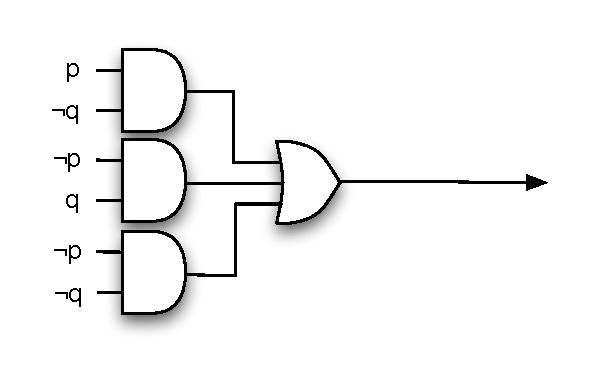
\epsfig{figure=Figures/fig-0-4.eps,width=\textwidth}}
\centerline{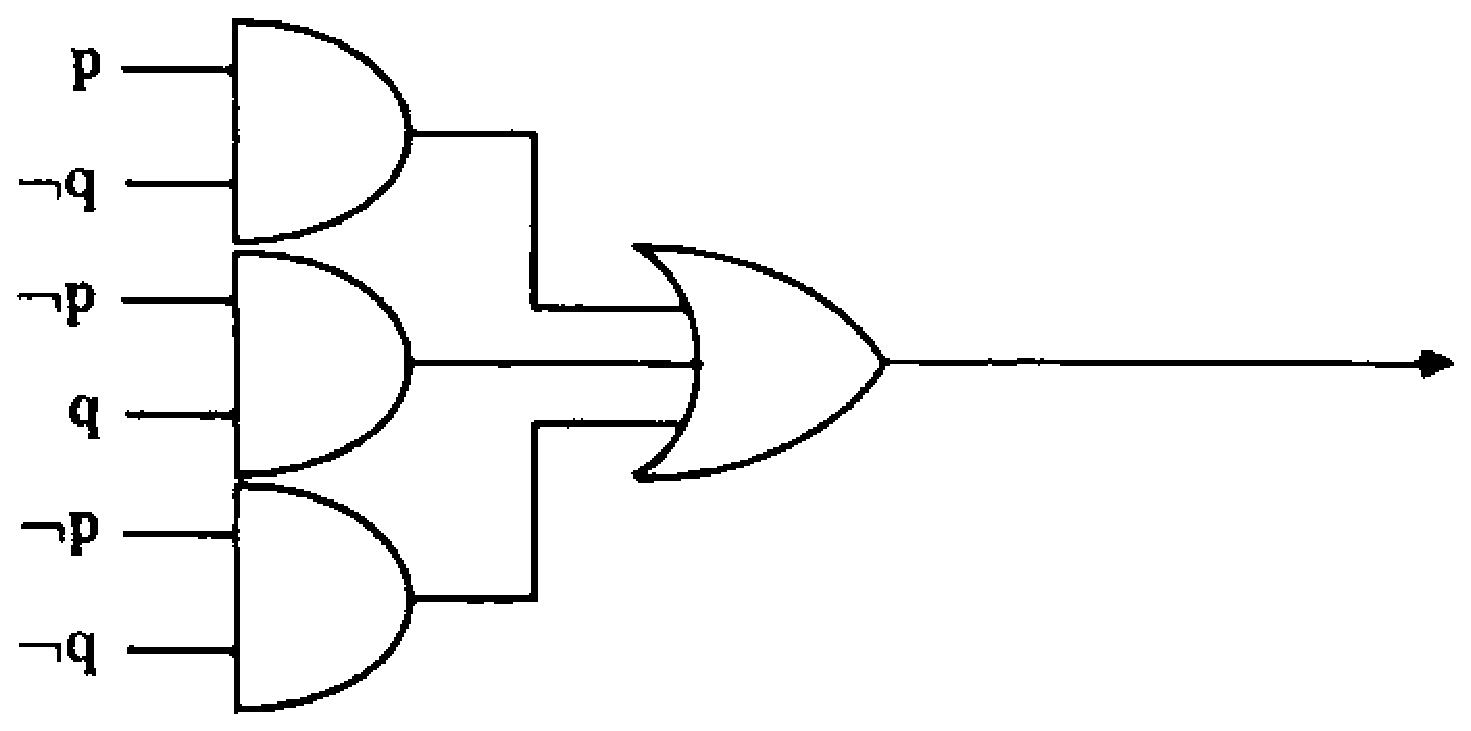
\epsfig{figure=ToFAfigures/fig0-4.eps,width=3.5in}}
\caption{A circuit equivalent to a single NAND gate}\label{fig-0.4}
\end{figure}

In a similar fashion, \emph{any} statement formula can be represented as a group of
AND gates feeding a single OR gate. In larger truth tables, there may
be many more $1$ values, and hence more complex statements may need many AND
gates. Regardless of the statement complexity, however, circuits based on the
PDNF of an expression will allow for a fast response to changing input signals,
since no signal must propagate through more than two gates.

Other useful equivalences are given in Figure \ref{fig-0.5}. Each rule has a \emph{dual}, written
on the same line.\index{associative law}\index{commutative law}\index{absorption law}\index{De Morgan's law}

% Figure 0.5
\begin{figure}[tb]
\begin{tabular}{r@{ $\Leftrightarrow$ }l@{$\qquad$}r@{ $\Leftrightarrow$ }l@{$\qquad$}l}
$(p \vee q) \wedge r$ & $(p \wedge r) \vee (q \wedge r)$ & $(p \wedge q) \vee r$
	& $(p \vee r) \wedge (q \vee r)$ & (distributive laws) \\
$(p \vee q) \vee r$ & $p \vee (q \vee r)$ & $(p \wedge q) \wedge r$ & $p \wedge
	(q \wedge r)$ & (associative laws) \\
$p \vee q$ & $q \vee p$ & $p \wedge q$ & $q \wedge p$ & (commutative laws) \\
$\neg (p \vee q)$ & $\neg p \wedge \neg q$ & $\neg (p \wedge q)$ & $\neg p \vee
	\neg q$ & (De Morgan's laws) \\
$(p \vee q) \wedge p$ & $p$ & $(p \wedge q) \vee p$ & $p$ & (absorption laws) \\
$p \vee \neg p$ & {\bf True} & $p \wedge \neg p$ & {\bf False} & (mutual
	exclusion)
\end{tabular}
\caption{Some useful equivalences and their duals}\label{fig-0.5}
\end{figure}

\emph{Predicates} are often used to make statements about certain \emph{objects}, such as
the numbers in the set ($\ZN$) of integers. For example, $Q$ might represent
the property of being less than 5, in which case $Q(x)$ will represent the
statement ``x is less than 5.'' Thus, $Q(3)$ is true, while $Q(7)$ is false. It
is often necessary to make global statements such as: \emph{All} integers have the
property $P$, which can be denoted by $(\forall x \in \ZN)P(x)$. Note that the
\emph{dummy} variable $x$ was used to state the concept in a convenient form; $x$ is
not meant to represent a particular object, and the statement could be
equivalently phrased as $(\forall i \in \ZN)P(i)$. For the predicate $Q$ defined
above, the statement $(\forall x \in \ZN)Q(x)$ is false, while when applied to
more restricted domains, $(\forall x \in\{1,2,3\})Q(x)$ is true, since it is in
this case equivalent to $Q(1) \wedge Q(2) \wedge Q(3)$, or $(1 < 5) \wedge (2 <
5) \wedge (3<5)$.

In a similar fashion, the statement that \emph{some} integers have the property $P$
will be denoted by $(\exists i\ \in\ \ZN)P(i)$. For the predicate $Q$ defined
above, $(\exists i\ \in \{4, 5, 6\})Q(i)$ is true, since it is equivalent to
$Q(4) \vee Q(5) \vee Q(6)$, or $(4 < 5) \vee (5 < 5) \vee (6 < 5).$ The
statement $(\exists y \in\{7, 8, 9\})Q(y)$ is false.

Note that asserting that it is not the case that all objects have the property
$P$ is equivalent to saying that there is at least one object that does not have
the property $P$. In symbols, we have
$$\neg(\forall x\in\ZN)P(x)\Leftrightarrow(\exists x\in\ZN)(\neg P(x))$$
Similarly,
$$\neg(\exists x\in\ZN)P(x)\Leftrightarrow(\forall x\in\ZN)(\neg P(x))$$
Given two statements $A$ and $B$, if $B$ is true whenever $A$ is true, we will
say that $A$ \emph{implies} $B$, and write $A \Rightarrow B$. For example, the
truth tables show that $p\wedge q\Rightarrow p\vee q$, since for the case where
$p\wedge q$ is true ($p=1,q=1$), $p\vee q$ is true, also. In the cases where $p
\wedge q$ is false, the value of $p\vee q$ is immaterial.

A basic knowledge of set theory is assumed. Some standard special symbols will
be repeatedly used to designate common sets.

% Definition 0.1
\begin{dfn}\label{dfn-0.1}
The set of {\em natural numbers\/} is given by $\NN = \{0,1,2,3,4, \ldots \}$.\index{natural numbers}\index{N @$\NN$|see{natural numbers}}

The set of {\em integers\/} is given by $\ZN =\{\ldots,-2,-1,0,1,2,\ldots\}$.\index{Z @$\ZN$ (integers)}

The set of {\em rational numbers\/} is given by $Q=\{\tfrac{a}{b}\ |\ a\in\ZN\wedge
b\in\ZN\wedge b\neq 0 \}$.\index{Q @$\QN$ (rationals)}

The set of {\em real numbers\/} (points on the number line) will be denoted by
$\RN$.\index{R @$\RN$ (reals)}
\end{dfn}

The following concepts and notation will be used frequently throughout the text.

% Definition 0.2.
\begin{dfn}\label{dfn-0.2}
Let $A$ and $B$ be sets. $A$ is a \emph{\Index{subset}} of $B$ if every element
of $A$ also belongs to $B$; that is, $A \subseteq B \Leftrightarrow (\forall x)
(x \in A \Rightarrow x \in B)$.
\end{dfn}

% Definition 0.3. 
\begin{dfn}\label{dfn-0.3}
Two sets $A$ and $B$ are said to be \emph{\Index{equal}} if they contain exactly
the same elements; that is, $A = B \Leftrightarrow (\forall x)(x \in A
\Leftrightarrow x \in B)$.
\end{dfn}

Thus, two sets $A$ and $B$ are equal \emph{iff} $A \subseteq B$ and $B \subseteq
A$. The symbol $\subset$ will be used to denote a \emph{proper} subset: 
$A \subset B$ \emph{iff} $A \subseteq B$ and $A \neq B$.\index{equality!of sets}

% Definition 0.4.
\begin{dfn}\label{dfn-0.4}
For sets $A$ and $B$, the \emph{\Index{cross product}}\index{Cartesian product|see{cross product}} of $A$ with $B$, is the
set of all ordered pairs from $A$ and $B$; that is, 
$A \times B = \{\langle a, b\rangle \ |\  a \in A \wedge b \in B\}$.
\end{dfn}

\section{Relations}\label{sec-0.2}
Relations are used to describe relationships between members of sets of objects.
Formally, a relation is just a subset of a cross product of two sets.

% Definition 0.5
\begin{dfn}\label{dfn-0.5}
Let $X$ and $Y$ be sets. A relation $R$ from $X$ to $Y$ is simply a
subset of $X \times Y$. If $\langle a,b\rangle \in R$, we write $aRb$. If
$\langle a,b\rangle\notin R$, we write $a$$\not\! R b$. If $X = Y$, we say $R$ is
a relation \underline{\emph{in}} X.
\end{dfn}

\subsection*{Example 0.2}

Let $X = \{1,2,3\}$. The familiar relation $<$ (less than) would then consist of
the following ordered pairs:
$<: \{\langle 1, 2\rangle , \langle 1, 3\rangle , \langle 2, 3\rangle \}$,
by which we mean to indicate that $1 < 2, 1 < 3$, and $2 < 3$.
$\langle 3,3\rangle \notin <$ since $3 \not< 3$.

Some relations have special properties. For example, the relation ``less than''
is \emph{transitive}, by which we mean that for any numbers $x, y,$ and $z,$
if $x < y$ and $y < z$, then $x < z$. Definition \ref{dfn-0.6} describes an important
class of relations that have some familiar properties.

% Definition 0.6
\begin{dfn}\label{dfn-0.6}
A relation is \emph{\Index{reflexive}} iff $(\forall x)(xRx)$.

A relation is \emph{\Index{symmetric}} iff $(\forall x)(\forall y)(xRy
	\Rightarrow yRx)$.

A relation is \emph{\Index{transitive}} iff $(\forall x)(\forall y)(\forall z)
	((xRy \wedge yRz) \Rightarrow x Rz).$
    
An \emph{equivalence relation} is a relation that is reflexive, symmetric, and
transitive.
\end{dfn}

\subsection*{Example 0.3}

\< is not an equivalence relation; while it is transitive, it is not reflexive
since $3 \not< 3$. (It is also not symmetric, since $2 < 3$, but $3 \not< 2$.)

\subsection*{Example 0.4}

Let $X = \NN$. The familiar relation $=$ (equality) \emph{is} an equivalence
relation.
$$= :\{\langle 0, 0\rangle , \langle 1,1\rangle , \langle 2,2\rangle ,
	\langle 3,3\rangle , \langle 4,4\rangle , \ldots \},$$
and it is clear that $(\forall x)(\forall y)(x = y \Rightarrow y = x)$.
The equality relation is therefore symmetric, and it is likewise obvious that
$=$ is also reflexive and transitive.

% Definition 0.7
\begin{dfn}\label{dfn-0.7}
Let $R$ be an equivalence relation in $X$, and let $h \in X$. Then $[h]_R$
refers to the \emph{equivalence class} consisting of all entities that are
related to $h$ by the equivalence relation $R$; that is, $[h]_R = \{y\ |\ y\ R\ h\}$.
\end{dfn}

\subsection*{Example 0.5}

The equivalence classes for $=$ are singleton sets: $[1]_==\{1\},[5]_==\{5\}$,
and so on.

\subsection*{Example 0.6}

Let $X = \ZN$, and define the relation $R$ in $\ZN\times\ZN$ by

$$\langle u, v\rangle R\langle w,x\rangle\ \text{{\em iff}}\ ux = vw$$

If $\langle x, y\rangle$ is viewed as the fraction $\frac{x}{y}$, then $R$ is
the relation that identifies equivalent fractions: $\frac{2}{3}R\frac{14}{21}$,
since $2\cdot 21=3\cdot 14$. In this sense, $R$ can be viewed as the \emph{equality}
operator on the set of rational numbers~$\QN$.\index{equality!of rationals}

Note that in this context the equivalence class $[\frac{2}{8}]_R$ represents the
set of all ``names'' for the point one-fourth of the way between $0$ and $1$;
that is,
$$\left[\frac{2}{8}\right]_R = \{\ldots ,\frac{-3}{-12}, \frac{-2}{-8},
\frac{-1}{-4}, \frac{1}{4},\frac{2}{8},\frac{3}{12},\frac{4}{16},\frac{5}{20},
\ldots \}$$
There are therefore many other ways of designating this same set; for example,
$$\left[\frac{1}{4}\right]_R = \{ \ldots , \frac{-3}{-12}, \frac{-2}{-8}, \frac{-1}{-4},
    \frac{1}{4},\frac{2}{8},\frac{3}{12},\frac{4}{16},\frac{5}{20}, \ldots \}$$

\subsection*{Example 0.7}

Let $X = \NN$ and choose an $n \in \NN$. Define $R_n$ by
$$x R_n y \text{\em { iff }}\, \, (\exists i \in \ZN)(x - y = i\cdot n)$$
That is, two numbers are related if their difference is a multiple of $n$.
Equivalently, $x$ and $y$ must have the same remainder upon dividing each of
them by $n$ if we are to have $x R_n y$
.
$R_n$ can be shown to be an equivalence relation for each natural number $n$.
The equivalence classes of $R_2$, for example, are the two familiar sets, the
even numbers and the odd numbers. The equivalence classes for $R_3$ are
\begin{center}\begin{tabular}{r@{ $=$ }l}
$[0]_{R_3}$ & $\{0, 3, 6, 9, 12, 15, \ldots \}$ \\
$[1]_{R_3}$ & $\{1, 4,7,10,13, \ldots \}$ \\
$[2]_{R_3}$ & $\{2, 5, 8,11,14, \ldots \}$
\end{tabular}\end{center}

$R_n$ is often called \emph{\Index{congruence modulo $n$}}, and $x R_n\!y$ is
commonly denoted by $x \equiv y\!\pmod{ n}$ or $x \equiv _n$$y$.

If $R$ is an equivalence relation in $X$, then every element of $X$ belongs to
exactly one equivalence class of $R$. $X$ is therefore comprised of the union of
the equivalence classes of $R$, and in this sense $R$ \emph{partitions} the set
$X$ into disjoint subsets. Conversely, a partition of $X$ defines an equivalence
relation in $X$; the sets of the partition can be thought of as the equivalence
classes of the resulting relation.

% Definition 0.8
\begin{dfn}\label{dfn-0.8}
Given a set $X$ and sets
$A_1 , A_2 , \ldots , A_n ,$ the collection $P = \{A_1 ,A_2 , \ldots ,A_n \}$
is a \emph{partition} of $X$ if the sets in $P$ are all \emph{subsets} of $X$,
they \emph{cover} $X$, and are \emph{pairwise disjoint}. That is, the following
three conditions are satisfied:

\begin{tabular}{r@{ $\in$ }l}
$(\forall i$ & $\{1,2, \ldots ,n\})(A_i \subseteq X)$ \\
$(\forall x$ & $X)(\exists i \in \{1,2, \ldots ,n\} \ni x \in A_i )$ \\
$(\forall i,j$ & $\{1, 2, \ldots ,n\})(i \not= j \Rightarrow A_i \cap A_j = \emptyset)$
\end{tabular}
\end{dfn}

% Definition 0.9
\begin{dfn}\label{dfn-0.9}
Given a set $X$ and a partition $P = \{A_1,A_2, \ldots ,A_n \}$ of $X$,
the relation $R(P)$ in $X$ induced by $P$ is given by
$$(\forall x \in X)(\forall y \in X)(x \, R(P) \, y \Leftrightarrow
  (\exists i \in \{1,2, \ldots ,n\} \ni x \in A_i \wedge y\in A_i))$$
\end{dfn}

$R(P)$ thus relates elements that belong to the same subset of $P$.

\subsection*{Example 0.8}

Let $X = \{1, 2, 3, 4, 5\}$ and consider the relation $Q = R(S)$ induced by the
partition $S = \{\langle 1, 2\rangle,\langle 3, 5\rangle,\langle 4\rangle\}$.
Since 1 and 2 are in the same set, they should be related by $Q$, while
$1$$\not\!\!\!Q 4$ because $1$ and $4$ belong to different sets of the partition.
Q can be described by
$$ Q = \{\langle 1, 1\rangle, \langle 1,2\rangle, \langle 2, 1\rangle,
\langle 2,2\rangle, \langle 3,3\rangle, \langle 3, 5\rangle,
\langle 4, 4\rangle, \langle 5, 3\rangle, \langle 5, 5\rangle\} $$

It is straightforward to check that $Q$ satisfies the three properties needed to
qualify as an equivalence relation, and the equivalence classes of $Q$ are
\begin{center}\begin{tabular}{r@{ $=$ }l}
$[1]_Q$ & $\{1,2\}$ \\
$[2]_Q$ & $\{1,2\}$ \\
$[3]_Q$ & $\{3,5\}$ \\
$[4]_Q$ & $\{4\}$ \\
$[5]_Q$ & $\{3,5\}$
\end{tabular}\end{center}

The set of \emph{distinct} equivalence classes of $Q$ can be used to partition
$X$; note that these three classes comprise $S$. In a similar manner, the three
distinct equivalence classes of $R_3$ in Example 0.7 form a partition of $\NN$.

A ``finer'' partition of $X$ can be obtained by breaking up the equivalence
classes of $Q$ into smaller (and hence more numerous) sets. The resulting
relation is called a \emph{refinement} of $Q$.

% Definition 0.10
\begin{dfn}\label{dfn-0.10}
Given two equivalence relations $R$ and $Q$ in a set $X$, $R$ is a
\emph{\Index{refinement}} of $Q\text{ iff }R \subseteq Q$; that is,
$(\forall x \in X)(\forall y \in X)(\langle x,y\rangle  \in R \Rightarrow \langle x,y\rangle  \in Q).$
\end{dfn}

\subsection*{Example 0.9}

Consider $Q = \{\langle 1, 1\rangle, \langle 1,2\rangle, \langle 2,1\rangle,
\langle 2,2\rangle, \langle 3,3\rangle, \langle 3,5\rangle, \langle 4,4\rangle,
\langle 5,3\rangle, \langle 5,5\rangle\}$
and $S =\{\langle 1, 1\rangle, \langle 2,2\rangle, \langle 3,3\rangle, \\
\langle 3,5\rangle, \langle 4,4\rangle, \langle 5,3\rangle,
\langle 5, 5\rangle\}$. $S$ is clearly a subset of $Q$, and hence $S$ refines
$Q$. Note that the partition induced by $S, \{\{1\}, \{2\}, \{3,5\},\{4\}\}$,
indeed splits up the partition induced by $Q$, which was
$\{\{1,2\},\{3,5\}, \{4\}\}$. While it may at first seem strange, the fact that
$S$ contained \emph{fewer} ordered pairs than $Q$ guarantees that $S$ will yield 
\emph{more} equivalence classes than $Q$.

\section{Functions}\label{sec-0.3}

A \emph{function} $f$ is a special type of relation in which each first
coordinate is associated with one and only one second coordinate, in which case
we can use functional notation $f(x)$ to indicate the unique element $f$
associates with a given first coordinate $x$. In the previous section we
concentrated on relations \emph{in} $X$, that is, subsets of $X \times X$. The
set of first coordinates of a function $f$ (the \emph{domain} $X$) is often
different from the set of possible second coordinates (the \emph{codomain} $Y$),
and hence $f$ will be a subset of $X \times Y$.

% Definition 0.11
\begin{dfn}\label{dfn-0.11}
A \emph{\Index{function}} f: $X \rightarrow Y$ is a subset of $X \times Y$ for
which 
\begin{enumerate}
\item $(\forall x \in X)(\exists y \in Y \ni xfy)$.
\item $(\forall x \in X)((xfy_1 \wedge xfy_2) \Rightarrow y_1 = y_2 )$.
\end{enumerate}
\end{dfn}

When a pair of elements are related by a function, we will write $f(a) = b$
instead of $afb$ or $\langle a,b\rangle\in f$. The criteria for being a function
could then be rephrased as $(\forall x \in X)(\exists y \in Y \ni f(x) = y)$,
and $(\forall x_1 \in X)(\forall x_2 \in X)(x_1 = x_2
\Rightarrow f(x_1) = f(x_2))$.

\subsection*{Example 0.10}

Let $n$ be a positive integer. Define $f_n$: $\NN \rightarrow \NN$ by $f_{n}(j)
=$ the smallest natural number $i$ for which $j \equiv i \bmod{n}, f_3 (j)$,
for example, is a function and is represented by the ordered pairs
$f_3: \{\langle 0, 0\rangle, \langle 1, 1\rangle, \langle 2, 2\rangle,
\langle 3, 0\rangle, \\ \langle 4,1\rangle, \ldots \}$. This implies that
$f_3 (0) = 0$, $f_3 (1) = 1$, $f_3 (2) = 2$, $f_3 (3) = 0$, and so on.

Note that $f_3$ is a subset of the relation $R_3$ given in Example 0.7. If $R_3$
were presented as a function, it would not be {\em well defined}; that is, $R_3$
does not satisfy Definition \ref{dfn-0.11}. For example, $2 R_3 5$ and $2 R_3 8$, but
$5 \not= 8$, and so $R_3 (2)$ is not a meaningful expression, since there is no
unique object that $R_3$ associates with 2. In this case, $R_3$ violated 
Definition \ref{dfn-0.11} by associating \emph{more} than one object with a
given first coordinate; in general, a proposed relation may also fail to be well
defined by associating \emph{no} objects with a potential first coordinate.

\subsection*{Example 0.11}

Consider the ``function'' $g$: $\QN \rightarrow \NN$ defined by $g(\frac{m}{n})
=m$. This apparently straightforward definition is fundamentally flawed.
According to the formula, $g\left(\frac{2}{8}\right)=2$, $g\left(\frac{7}{9}
\right)=7$, $g\left(\frac{5}{10}\right)=5$, and so forth. However, $\frac{2}{8}
=\frac{5}{20}$, but $g\left(\frac{2}{8}\right)=2\not=5=g\left(\frac{5}{20}
\right)$, and Definition \ref{dfn-0.11} is again violated; $g(0.25)$ is not a
well defined quantity, and thus the ``function'' $g$ is not well defined. Had
$g$ truly been a function, it would have passed the test: if $x=y$, then $g(x)=
g(y)$.

The problem with this seemingly innocent definition
is that the domain element 0.25 is actually
an {\em equivalence class} of fractions (recall Example 0.6), and the definition
of $g$ was based on just one \emph{representative} of that class. We observed
that two representatives ($\frac{2}{8}$ and $\frac{5}{20}$) of the \emph{same}
class gave conflicting answers (2 and 5) for the value that $g$ associated with
their class (0.25). While it is possible to define functions on a set of
equivalence classes in a consistent manner, it will always be important to
verify that such functions are {\em single valued}.

Selection criteria, which determine whether a candidate does or does not
belong to a given set, are special types of functions.

% Definition 0.12
\begin{dfn}\label{dfn-0.12}
Given a set $A$, the {\em characteristic function} $\chi_A$ associated with $A$
is defined by
$$\chi_{A}(x)=1\text{ if }x\in A\quad\text{and}\quad\chi_{A}(x)=0\text{ if }x
	\notin A$$
\end{dfn}

\subsection*{Example 0.12}

The characteristic function for the set of odd numbers is the function $f_2$
given in Example 0.10.

To say that a \emph{set} is well defined essentially means that the
characteristic function associated with that set is a well-defined function. A
set of equivalence classes can be ill defined if the definition is based on the
representatives of those equivalence classes.

\subsection*{Example 0.13}

Consider the ``set'' of fractions that have odd numerators, whose characteristic
``function'' is defined by:
$$\chi_{B}\left(\frac{m}{n}\right) = 1\text{ if $m$ is odd}$$
and
$$\chi_{B}\left(\frac{m}{n}\right) = 0\text{ if $m$ is even}$$

This characteristic function suffers from flaws similar to those found in the
function $g$ in Example 0.11. $\frac{1}{4} = \frac{2}{8}$ and yet
$X_B \left(\frac{1}{4}\right) = 1$ while $X_B \left(\frac{2}{8}\right) = 0$,
which implies that the fraction $\frac{1}{4}$ belongs to $B$, while
$\frac{2}{8}$ is not an element of $B$. Due to this ambiguous definition of set
membership, $B$ is not a well-defined set. $B$ failed to pass the test: if
$x = y$, then $(x \in B$ \emph{iff} $y\in B)$.

The definition of a relation requires the specification of the domain, codomain,
and the ordered pairs comprising the relation. For relations that are functions,
every domain element must occur as a first coordinate. However, the set of
elements that occur as second coordinates need not include all the codomain
(as was the case in the function $f_n$ in Example 0.10).

% Definition 0.13
\begin{dfn}\label{dfn-0.13}
The \emph{\Index{range}} of a function $f: X \rightarrow Y$ is given by
$$\{y \in Y\ |\  \exists x \in X \ni f(x) = y\}$$
\end{dfn}

Conditions similar to those imposed on the behavior of first coordinates of a
function may also be placed on second coordinates, yielding specialized types
of functions. Functions for which the range encompasses all the codomain, for
example, are called \emph{surjective}

% Definition 0.14
\begin{dfn}\label{dfn-0.14}
A function $f$: $X \rightarrow Y$ is \emph{\Index{onto}} or
\emph{\Index{surjective}} iff
$$(\forall y \in Y)(\exists x \in X \ni  f(x) = y)\text{; that is,}$$
a set of ordered pairs representing an \emph{onto} function must have at least
one first coordinate associated with any given second coordinate .
\end{dfn}

\subsection*{Example 0.14}

The function $g$: $\{1,2,3\}\rightarrow\{a,b\}$ defined by $g(1) = a$,
$g(2) = b$, and $g(3) = a$ is onto since both codomain elements are part of the
range of $g$. However, the function $h$: $\{1, 2, 3\}\rightarrow \{a, b, c\}$
defined by $h(1) = a$, $h(2) = b$, and $h(3) = a$ is \emph{not} onto since no domain
element maps to $c$.

The function $f$: $\NN \rightarrow \NN$ defined by $f(i)=i+1$ $(\forall i=0,1,2,
\ldots)$ is \emph{not} onto since there is no element $x$ for which $f(x)=0$.

% Definition 0.15
\begin{dfn}\label{dfn-0.15}
A function $f$: $X \rightarrow Y$ is \emph{\Index{one to one}} or
\emph{\Index{injective}} iff
$$(\forall x_1 \in X)(\forall x_2 \in X)(f(x_1) = f(x_2)
	\Rightarrow x_1 = x_2)\text{; that is,}$$
an \emph{injective} function must not have more than one first coordinate
associated with any given second coordinate .
\end{dfn}

\subsection*{Example 0.15}

The function $f$: $\NN \rightarrow \NN$ defined by $f(i)=i+1$ $(\forall i=0,1,2,
\ldots)$ is clearly injective since if $f(i)= f(j)$ then $i+1=j+1$, and so $i$
must equal $j$.

The function $g$: $\{1,2,3\}\times\{a,b\}$ defined by $g(1)=a$, $g(2)=b$,
and $g(3)=a$ is not one to one since $g(1)=g(3)$, but $1\not= 3$.

% Definition 0.16
\begin{dfn}\label{dfn-0.16}
A function is a \emph{\Index{bijection}} iff it is one to one and onto
(injective and surjective); that is, it must satisfy
\begin{enumerate}
\item $(\forall x_1 \in X)(\forall x_2 \in X)(f(x_1) = f(x_2) \Rightarrow x_1 =
	x_2)$.
\item $(\forall y \in Y)(\exists x \in X \ni f(x) = y)$.
\end{enumerate}
\end{dfn}

A \emph{bijective} function must therefore have \emph{exactly} one first
coordinate associated with any given second coordinate.

\subsection*{Example 0.16}

The function $f$: $\NN \rightarrow \NN$ defined by $f(i)=i+1$ $(\forall i=0,1,2,
\ldots)$ is injective but not surjective, so it is not a bijection. However, the
function $b$: $\ZN\rightarrow\ZN$ defined by $b(i)=i+1$ $(\forall i=\ldots,-2,
-1,0,1,2,\ldots)$ is a bijection. Note that while the rule for $b$ remains the
same as for $f$, both the domain and range have been expanded, and many more
ordered pairs have been added to form the function $b$.

It is often appropriate to take the results produced by one function and apply
the rule specified by a second function. For example, we may have a list
associating students with their height in inches (that is, we have a function
relating names with numbers). The conversion rule for changing inches into
centimeters is also a function (associating any given number of inches with the
corresponding length in centimeters), which can be applied to the heights given
in the student list to produce a new list matching student names with their
height in centimeters. This new list is referred to as the
\emph{\Index{composition}} of the original two functions.

% Definition 0.17
\begin{dfn}\label{dfn-0.17}
The \emph{\Index{composition}} of two functions $f$: $X\rightarrow Y$ and
$g$: $Y\rightarrow Z$ is given by
$$g \circ f = \{\langle x,z\rangle \ |\  \exists y \in Y \ni
	\langle x,y\rangle \in f\text{ and }\langle y,z\rangle \in g\}$$
\end{dfn}

Note that the composition is not defined unless the codomain of the first
function matches the domain of the second function. In functional notation,
$g\circ f=\{\langle x,z\rangle\ |\ \exists y\in Y\ni f(x)=y\text{ and }g(y)=z\}$,
and therefore when $g\circ f$ is defined, it can be described by the rule
$g\circ f(x)=g(f(x))$.

\subsection*{Example 0.17}

Consider the functions $f_3$ from Example 0.10 and $f$ from Example 0.14, where
$f_3$: $\NN\rightarrow\NN$ was defined by $f_3(i) =$ the smallest natural number
$i$ for which $j = i \bmod{3}$, and the function $f$: $\NN\rightarrow\NN$ is
defined by $f(i) = i + 1$. $f \circ f_3$ consists of the ordered pairs
$\{\langle 0,1\rangle,\langle 1,2\rangle,\langle 2,3\rangle,\langle 3,1\rangle,
\langle 4,2\rangle,\langle 5,3\rangle, \ldots \}$ and is represented by the rule
$f\circ f_3(j) = f_3(j) + 1$, which happens to be the smallest {\em positive}
number that is congruent to $j + 1 \bmod{3}$. Note that
$f_3 \circ f(j) = f_3 (j + 1)$, which happens to be the smallest \emph{natural}
number that is congruent to $j + 1 \bmod{3}$. This represents a different set
of ordered pairs $\{\langle 0,1\rangle,\langle 1,2\rangle,\langle 2,0\rangle,
\langle 3,1\rangle,\langle 4,2\rangle,\langle 5,0\rangle, \ldots \}$. In most
cases, $f \circ g \not= g \circ f$.

% Theorem 0.1
\begin{thm}\label{thm-0.1}
Let the functions $f$: $X\rightarrow Y$ and $g$: $Y\rightarrow Z$ be onto. Then
$g\circ f$ is onto.

\emph{Proof.} See the exercises.
\end{thm}

% Theorem 0.2
\begin{thm}\label{thm-0.2}
Let the functions $f$: $X\rightarrow Y$ and $g$: $Y\rightarrow Z$ be one to one.
Then $g\circ f$ is one to one.

\emph{Proof.} See the exercises.
\end{thm}

% Definition 0.18
\begin{dfn}\label{dfn-0.18}
The \emph{\Index{converse}} of a relation $R$, written $\sim\! R$, is defined by
$$\sim\! R = \{\langle y,x\rangle \ |\  \langle x,y\rangle \in R\}$$
The converse of a function $f$ is likewise
$$\sim\!\! f = \{\langle y,x\rangle \ |\  \langle x,y\rangle \in f\}$$
If $\sim\!\! f$ happens to be a function, it is called the \emph{inverse} of $f$ and
is denoted by $f^{-1}$.
\end{dfn}

When the inverse exists, it is appropriate to use functional notation $f^{-1}$
also, and we therefore have, for any elements $a$ and $b$, $f^{-1}(b) = a$
{\em iff} $f(a) = b$. Note that if $f: X \rightarrow Y$ then
$f^{-1}: Y \rightarrow X$.

\subsection*{Example 0.18}

Consider the ordered pairs for the relation
$<: \{\langle 1,2\rangle,\langle 1,3\rangle,\langle 2,3\rangle\}$. The converse
is then $\sim <: \{\langle 2,1\rangle,\langle 3,1\rangle,\langle 3,2\rangle \}$.
Thus, the converse of ``less than'' is the relation ``greater than''

The function $b$:$\ZN \rightarrow \ZN$ defined by
$b(i) = i + 1 (\forall i = \ldots,-2, -1,0,1,2, \ldots)$ has the inverse
$b^{-1}: \ZN \rightarrow \ZN$ defined by
$b^{-1}(i) = i - 1 (\forall i = \ldots,-2,-1,0,1,2,\ldots)$. The inverse of the
function that increments integers by 1 is the function that decrements integers
by the same amount.

The function $f$: $\ZN \rightarrow \ZN$ defined by
$f(i) = i^2 (\forall i = \ldots,-2,-1,0,1,2,\ldots)$ has a converse that is not
a function over the given domain and codomain; the inverse notation is
inappropriate, since $f^{-1}(3)$ is not defined, nor is $f^{-1}(-4)$.

Not surprisingly, if the converse of $f$ is to be a function, the codomain of
$f$ (which will be the new domain of $f^{-1}$) must satisfy conditions similar
to those imposed on the domain of $f$. In particular:

% Theorem 0.3
\begin{thm}\label{thm-0.3}
Let $f$: $X\rightarrow Y$ be a function. The converse of $f$ is a function iff
$f$ is a bijection.

\emph{Proof}. See the exercises.
\end{thm}

If $f$ is a bijection, $f^{-1}$ must exist and will also be a bijection. In
fact, the compositions $f \circ f^{-1}$ and $f^{-1} \circ f$ are the
\emph{identity} functions on the domain and codomain, respectively (see the
exercises).

\section{Cardinality and Induction}\label{sec-0.4}

The \emph{size} of various sets will frequently be of interest in the topics
covered in this text, and it will occasionally be necessary to consider the set
of all subsets of a given set.

% Definition 0.19
\begin{dfn}\label{dfn-0.19}
Given a set $A$, the \emph{\Index{power set}} of $A$, denoted by $\wp (A)$ or
$2^A$, is $$\wp(A) = \{X\ |\ X \subseteq A\}$$
\end{dfn}

\subsection*{Example 0.19}

$$\wp(\{a,b,c\}) =
	\{\emptyset,\{a\},\{b\},\{c\},\{a,b\},\{a,c\},\{b,c\},\{a,b,c\}\}$$
and
$$\wp(\{\ \ \})=\{\emptyset\}.$$
Note that $\{\emptyset\} \not= \emptyset$.

% Definition 0.20
\begin{dfn}\label{dfn-0.20}
Two sets $X$ and $Y$ are \emph{\Index{equipotent}} if there exists a bijection
$f$: $X \rightarrow Y$, and we will write $\| X\| = \| Y\|.\ \ \| X\|$ denotes the
\emph{\Index{cardinality}} of $X$, that is, the number of elements in $X$.
\end{dfn}

That is, sets with the same cardinality or ``size'' are equipotent. The
equipotent relation is reflexive, symmetric, and transitive and is therefore an
equivalence relation.

\subsection*{Example 0.20}

The function $g$: $\{a,b,c\}\rightarrow\{x,y,z\}$ defined by $g(a)=z$, $g(b)=y$,
and $g(c)=x$ is a bijection, and thus $\|\{a,b,c\}\|=\|\{x,y,z\}\|$. The
equivalence class consisting of all sets that are equipotent to $\{a,b,c\}$ is
generally associated with the \emph{cardinal number} 3. Thus, $\|\{a,b,c\}\| =
3$; $\|\{\ \ \}\|=0$. $\{a,b,c\}$ is not equipotent to $\{\ \ \}$, and hence $3
\not= 0$.

The subset relation allows the sizes of sets to be \emph{ordered}:
$\|A\| \leq \|B\|$ {\em iff} $(\exists C)(C \subseteq B \wedge \|A\| = \|C\|)$.
We will write 
$\|A\| < \|B\|$ {\em iff} $(\|A\| \leq \|B\|\text{ and }\|A\| \not= \|B\|)$.
The observations about $\{a,b,c\}$ and $\{\ \}$ imply that $0 < 3$.

For $\NN =\{0,1,2,3,4,5,6, \ldots \}$ and $\EN =\{0,2,4,6, \ldots \}$, the
function $f$: $\NN \rightarrow \EN$, defined by $f(x) = 2x$, is a bijection. The
set of natural numbers $\NN$ is \emph{countably infinite}, and its size is often
denoted by $\aleph_0= \|\NN\|$. The doubling function $f$ shows that
$\|\NN\| = \|\EN\|$. Similarly, it can be shown that $\ZN$ and $\NN \times \NN$
are also countably infinite (see the exercises). A set that is equipotent to one
of its {\em proper} subsets is called an infinite set. Since $\|\NN\| = \|\EN\|$ and
yet $\EN \subset \NN$, we know that $\NN$ must be infinite. No such
correspondence between $\{a,b,c\}$ and any of its proper subsets is possible, so
$\{a,b,c\}$ is a finite set. 3 is therefore a finite cardinal number, while
$\aleph_0$ represents an infinite cardinal number.

Theorem \ref{thm-0.4} compares the size of a set $A$ with the number of subsets of $A$ and
shows that $\|A\| < \|\wp(A)\|$. For the sets in Example 0.19, we see that
$3 < 8$ and $0 < 1$, which is not unexpected. It is perhaps surprising to find
that the theorem will also apply to infinite sets, for example,
$\|\NN\| < \|\wp(\NN)\|$. This means that there are cardinal numbers larger
than $\aleph_0$; there are infinite sets that are not countably infinite.
Indeed, the next theorem implies that there is an unending progression of
infinite cardinal numbers.

% Theorem 0.4
\begin{thm}\label{thm-0.4}
Let A be \emph{any} set. Then $\|A\| < \|\wp(A)\|$

\emph{Proof}. There is a bijection between $A$ and the set of all singleton
subsets of $A$, as shown by the function $s$: $A \rightarrow \{\{x\}\ |\ x \in A\}$
defined by $s(z) = \{z\}$ for each $z \in A$. Since
$\{\{x\}\ |\ x\in A\}\subseteq \wp(A)$, we have $\|A\| \leq \|\wp(A)\|$. It
remains to show that $\|A\| \not= \|\wp(A)\|$. By definition of cardinality, we
must show that there cannot exist a bijection between $A$ and $\wp(A)$. The
following proof by contradiction will show this.

Assume $f$: $A\rightarrow \wp(A)$ is a function; we will demonstrate that there
must exist a set in $\wp(A)$ that is not in the range of $f$, and hence $f$
cannot be onto. Consider an element $z$ of $A$ and the set $f(z)$ to which it
maps. $f(z)$ is a subset of $A$, and hence $z$ may or may not belong to $f(z)$.
Define $B$ to be the set $\{y \in A \ |\  y \notin f(y)\}$. $B$ is then the set of
all elements of $A$ that do not appear in the set corresponding to their image
under $f$. It is impossible for $B$ to be in the range of $f$, for if it were
then there would be an element of $A$ that maps to this subset: assume $w \in A$
and $f(w) = B$. Since $w$ is an element of $A$, it might belong to $B$, which is
a subset of $A$. If $w \in B$, then $w \in f(w)$, since $f(w) = B$; but the
elements for which $y \in f(y)$ were exactly the ones omitted from $B$, and thus
we would have $w \notin B$, which is a contradiction. Our speculation that $w$
might belong to $B$ is therefore incorrect. The only other option is that $w$
does not belong to $B$. But if $w \notin B = f(w)$, then $w$ is one of the
elements that are supposed to be in $B$ and we are again faced with the
impossibility that $w \notin B$ and $w \in B$. In all cases, we reach a
contradiction if we assume that there exists an element $w$ for which $f(w) = B$.
Thus, $B$ was a member of the codomain that is not in the range of $f$, and $f$ 
is therefore not a bijection.
\end{thm}

Sets that are finite or are countably infinite are called
\emph{\Index{countable}} or \emph{\Index{denumerable}} because their elements can be
arranged one after the other (enumerated). We will often need to prove that a
given statement is true in an infinite variety of cases that can be enumerated
by the natural numbers $0,1,2,\ldots$. The assertion that the sum of the first
$n$ positive numbers can be predicted by multiplying $n$ by the number one
larger than $n$ and dividing the result by 2 seems to be true for various test
values of $n$:
\begin{center}\begin{tabular}{r@{ $=$ }l}
$1+2+3$ & $\frac{(3+1)3}{2}$ \\
$1+2+3+4+5$ & $\frac{(5+1)5}{2}$
\end{tabular}\end{center}
and so on. We would like to show that the assertion is true for all values of
$n = 1,2,3, \ldots$, but we clearly could never check the arithmetic
individually for an infinite number of cases. The assertion, which varies
according to the particular number $n$ we choose, can be represented by the
statement
$$P(n)\text{:}\ 1+2+3+\cdots+(n-2)+(n-1)+n\text{ adds up to }\frac{(n+1)n}{2}.$$
Note that $P(n)$ is \emph{not} a number; it is the assertion that two numbers are the
same and therefore will only take on the values {\bf True} and {\bf False}. We
would like to show that $P(n)$ is true for each positive integer $n$; that is,
$(\forall n)P(n)$. Notice that if you were to attempt to check out whether
$P(101)$ was true your work would be considerably simplified if you already knew
how the first 100 numbers added up. If the first 100 summed to 5050, it is clear
that $1+2+\cdots+99+100+101=(1+2+\cdots+99+100)+101=5050+101=5151$; the hard
part of the calculation can be done \emph{without} doing arithmetic with 101
separate numbers. Checking that $\frac{(101+1)101}{2}$ agrees with 5151 shows
that $P(101)$ is indeed true [that is, as long as we are sure that our
calculations in verifying $P(100)$ are correct]. Essentially, the same technique
could have been used to show that $P(6)$ followed from $P(5)$. This trick of
using the results of previous cases to help verify further cases is reflected in
the principle of mathematical induction.

% Theorem 0.5
\begin{thm}\label{thm-0.5}
Let $P(n)$ be a statement for each natural number $n \in \NN$. From the two
hypotheses
\begin{enumerate}[i.]
\item $P(0)$
\item $(\forall m \in \NN)(P(m) \Rightarrow P(m + 1))$
\end{enumerate}
we can conclude $(\forall n \in \NN)P(n)$.
\end{thm}

The fundamental soundness of the principle is obvious in light of the following
analogy: Assume you can reach the basement of some building (hypothesis i). If
you were assured that from \emph{any} floor $m$ you could reach the next higher
floor (hypothesis ii), you would then be assured that you could reach any floor
you wished $((\forall n \in \NN)P(n))$.

Similar statements can be made from other starting points; for example,
beginning with $P(4)$ and $(\forall m$$>$$4)(P(m) \Rightarrow P(m + 1)$, we can
derive the conclusion $(\forall m > 4)P(n)$; had we started on the fourth floor
of the building, we could reach \emph{any} of the higher floors.

\subsection*{Example 0.21}

Consider the statement discussed above, where $P(n)$ was the assertion that
$1 + 2 + 3 + \cdots + (n - 2) + (n - 1) + n$ adds up to $\frac{(n + 1)n}{2}$. We
will begin with $P(1)$ (the \emph{basis} step)\index{basis step} and note that
$1=\frac{(1 + 1)1}{2}$, so $P(1)$ is indeed true. For the \emph{inductive} step, let
$m$ be an arbitrary (but fixed) positive integer, and assume $P(m)$ is true;
that is, $1 + 2 + 3 + \cdots + (m - 2) + (m - 1) + m$ adds up to
$\frac{(m + 1)m}{2}$. We need to show
$P(m+1)$: $1+2+3+\cdots+(m+1-2)+(m+1-1)+(m+1))$ adds up to $\frac{(m+1+1)(m+1)}
{2}$. As in the case of proceeding from 100 to 101, we will use the fact that
the first $m$ integers add up correctly (the induction assumption) to see how
the first $m+1$ integers add up. We have:
\begin{center}\begin{tabular}{r@{ }l}
$1+2+3+\cdots+(m+1$ & $-2)+(m+1-1)+(m+1)$ \\
& $=(1+2+3+\cdots+(m+1-2)+(m+1-1))+(m+1)$ \\
& $=\frac{(m + 1)m}{2} + (m + 1)$ \\
& $=\frac{(m + 1)m}{2} + \frac{(m + 1)2}{2}$ \\
& $=\frac{((m + 1)m + (m + 1)2)}{2}$ \\
& $=\frac{(m + 1)(m + 2)}{2}$ \\
& $=\frac{(m + 1 + 1)(m + 1)}{2}$
\end{tabular}\end{center}

$P(m+1)$ is therefore true, and $P(m + 1)$ indeed follows from $P(m)$. Since $m$
was arbitrary, $(\forall m)(P(m) \Rightarrow P(m + 1))$ and, by induction,
$(\forall n \geq 1)P(n)$. The formula is therefore true for every positive
integer $n$. It is interesting to note that, with the usual convention of
defining the sum of \emph{no} integers to be zero, the formula also holds for $n = 0$,
and $P(0)$ could have been used as the basis step to prove
$(\forall n \in \NN)P(n)$.

\subsection*{Example 0.22}

Consider the statement
\begin{quote}
Any statement formula using the $n$ variables $p_1, p_2, \ldots , p_n$ has an
equivalent expression that contains less than $n \cdot 2^n$ operators.
\end{quote}
This can be proved by induction on the statement
\begin{quote}\index{equivalent!logical expressions}
$P(n):$ Any statement formula using $n$ or \emph{fewer} variables has an
equivalent expression that contains less than $n \cdot 2^n$ operators.
\end{quote}

\emph{Basis step:} A statement formula in one variable must be either be
$p$, $\neg p$, {\bf T}, or {\bf F}, each of which requires at most one
operator, and since $1<1\cdot 2^1$, $P(1)$ is true.

\emph{Inductive step:} Assume $P(m)$ is true; we need to prove that $P(m + 1)$
is true, which is to say that we need to ensure that the statement holds not
just for formulas with $m$ or fewer variables, but also for formulas with $m+1$
variables. Thus, choose an expression $S$ containing the variables
$p_1, p_2, \ldots ,p_m, p_{m+1}$. Consider the principal disjunctive normal form
(PDNF) of $S$. This expression is equivalent to $S$ and has terms that can be
separated into two categories: (1) those that contain the term $p_{m+1}$, and
(2) those that contain the term $\neg p_{m+1}$. While the PDNF may very well
contain more than the desired number of terms, the distributive law can be used
to factor $p_{m+1}$ out of all the terms in (1), leaving an expression of the
form $C \wedge p_{m+1}$ where $C$ is a formula containing only the terms
$p_1, p_2, \ldots, p_m$. Similarly, $\neg p_{m+1}$ can be factored out of all
the terms in (2), leaving an expression of the form $D \wedge \neg p_{m+1}$,
where D is also a formula containing only the terms $p_1, p_2, \ldots, p_m$.

$S$ can therefore be written as $(C \wedge p_{m+1})\vee(D \wedge \neg p_{m+1})$,
which contains the four operators $\wedge, \vee, \wedge$, and $\neg$ and the
operators that comprise the formulas for C and D. However, since both C and D
only contain the $m$ variables $p_1, p_2, \ldots, p_m$, the induction assumption
ensures that they each have equivalent representations using no more than
$m \cdot 2^m$ operators. $S$ can therefore be written in a form containing at
most $4 + m \cdot 2^m + m \cdot 2^m$ operators, which can be shown to be less
than $(m + 1)\cdot 2^{m+1}$ for all positive numbers $m$. Since $S$ was an
arbitrary expression with $m + 1$ operators, we have shown that $any$ statement
formula using exactly $m + 1$ variables has an equivalent expression that
contains no more than $(m + 1) \cdot 2^{m + 1}$ operators.

Since $P(m)$ was assumed true, we likewise know that any statement formula
using $m$ or fewer variables also has an equivalent expression that contains no
more than $m \cdot 2^m$ operators. $P(m + 1)$ is therefore true, and $P(m + 1)$
indeed follows from $P(m)$. Since $m$ was an arbitrary positive integer,
$(\forall m > 1)(P(m) \Rightarrow P(m + 1))$ and by induction
$(\forall n > 1)P(n)$. The formula is therefore true for every natural number
$n$.

\section{Recursion}\label{sec-0.5}

Since this text will be dealing with devices that repeatedly perform certain
operations, it is important to understand the recursive definition of functions
and how to effectively investigate the properties of such functions. Recall that
the factorial function ($f(n) = n!$) is defined to be the product of the first
$n$ integers. Thus,
\begin{center}\begin{tabular}{r@{ $=$ }l}
$f(1)$ & $1$ \\
$f(2)$ & $1\cdot 2=2$ \\
$f(3)$ & $1\cdot 2\cdot 3=6$ \\
$f(4)$ & $1\cdot 2\cdot 3\cdot 4=24$
\end{tabular}\end{center}
and so on. Note that individual definitions get longer as $n$ increases. If we
adopt the convention that $f(0) = 1$, the factorial function can be \emph{recursively}
defined in terms of other values produced by the function.

% Definition 0.21
\begin{dfn}\label{dfn-0.21}
For $x \in \NN$, define
\begin{center}\begin{tabular}{ll}
$f(x) = 1$, & if $x = 0$ \\
$f(x) = x \cdot f(x-1)$, & if $x > 0$
\end{tabular}\end{center}
\end{dfn}

This definition implies that
$f(3)=3\cdot f(2) = 3\cdot 2\cdot f(1) = 3\cdot 2\cdot 1\cdot f(0) =
	3\cdot 2\cdot 1\cdot 1=6$.

% 0.6 BACKUS-NAUR FORM
\section{Backus-Naur Form}\label{sec-0.6}
The syntax of programming languages is often illustrated with
{\em \Index{syntax diagrams}} or described in {\em Backus-Naur Form (\Index{BNF}})\index{Backus-Naur Form|see{BNF}} notation.

\begin{figure}[tb]
% Figure 0.6
\centerline{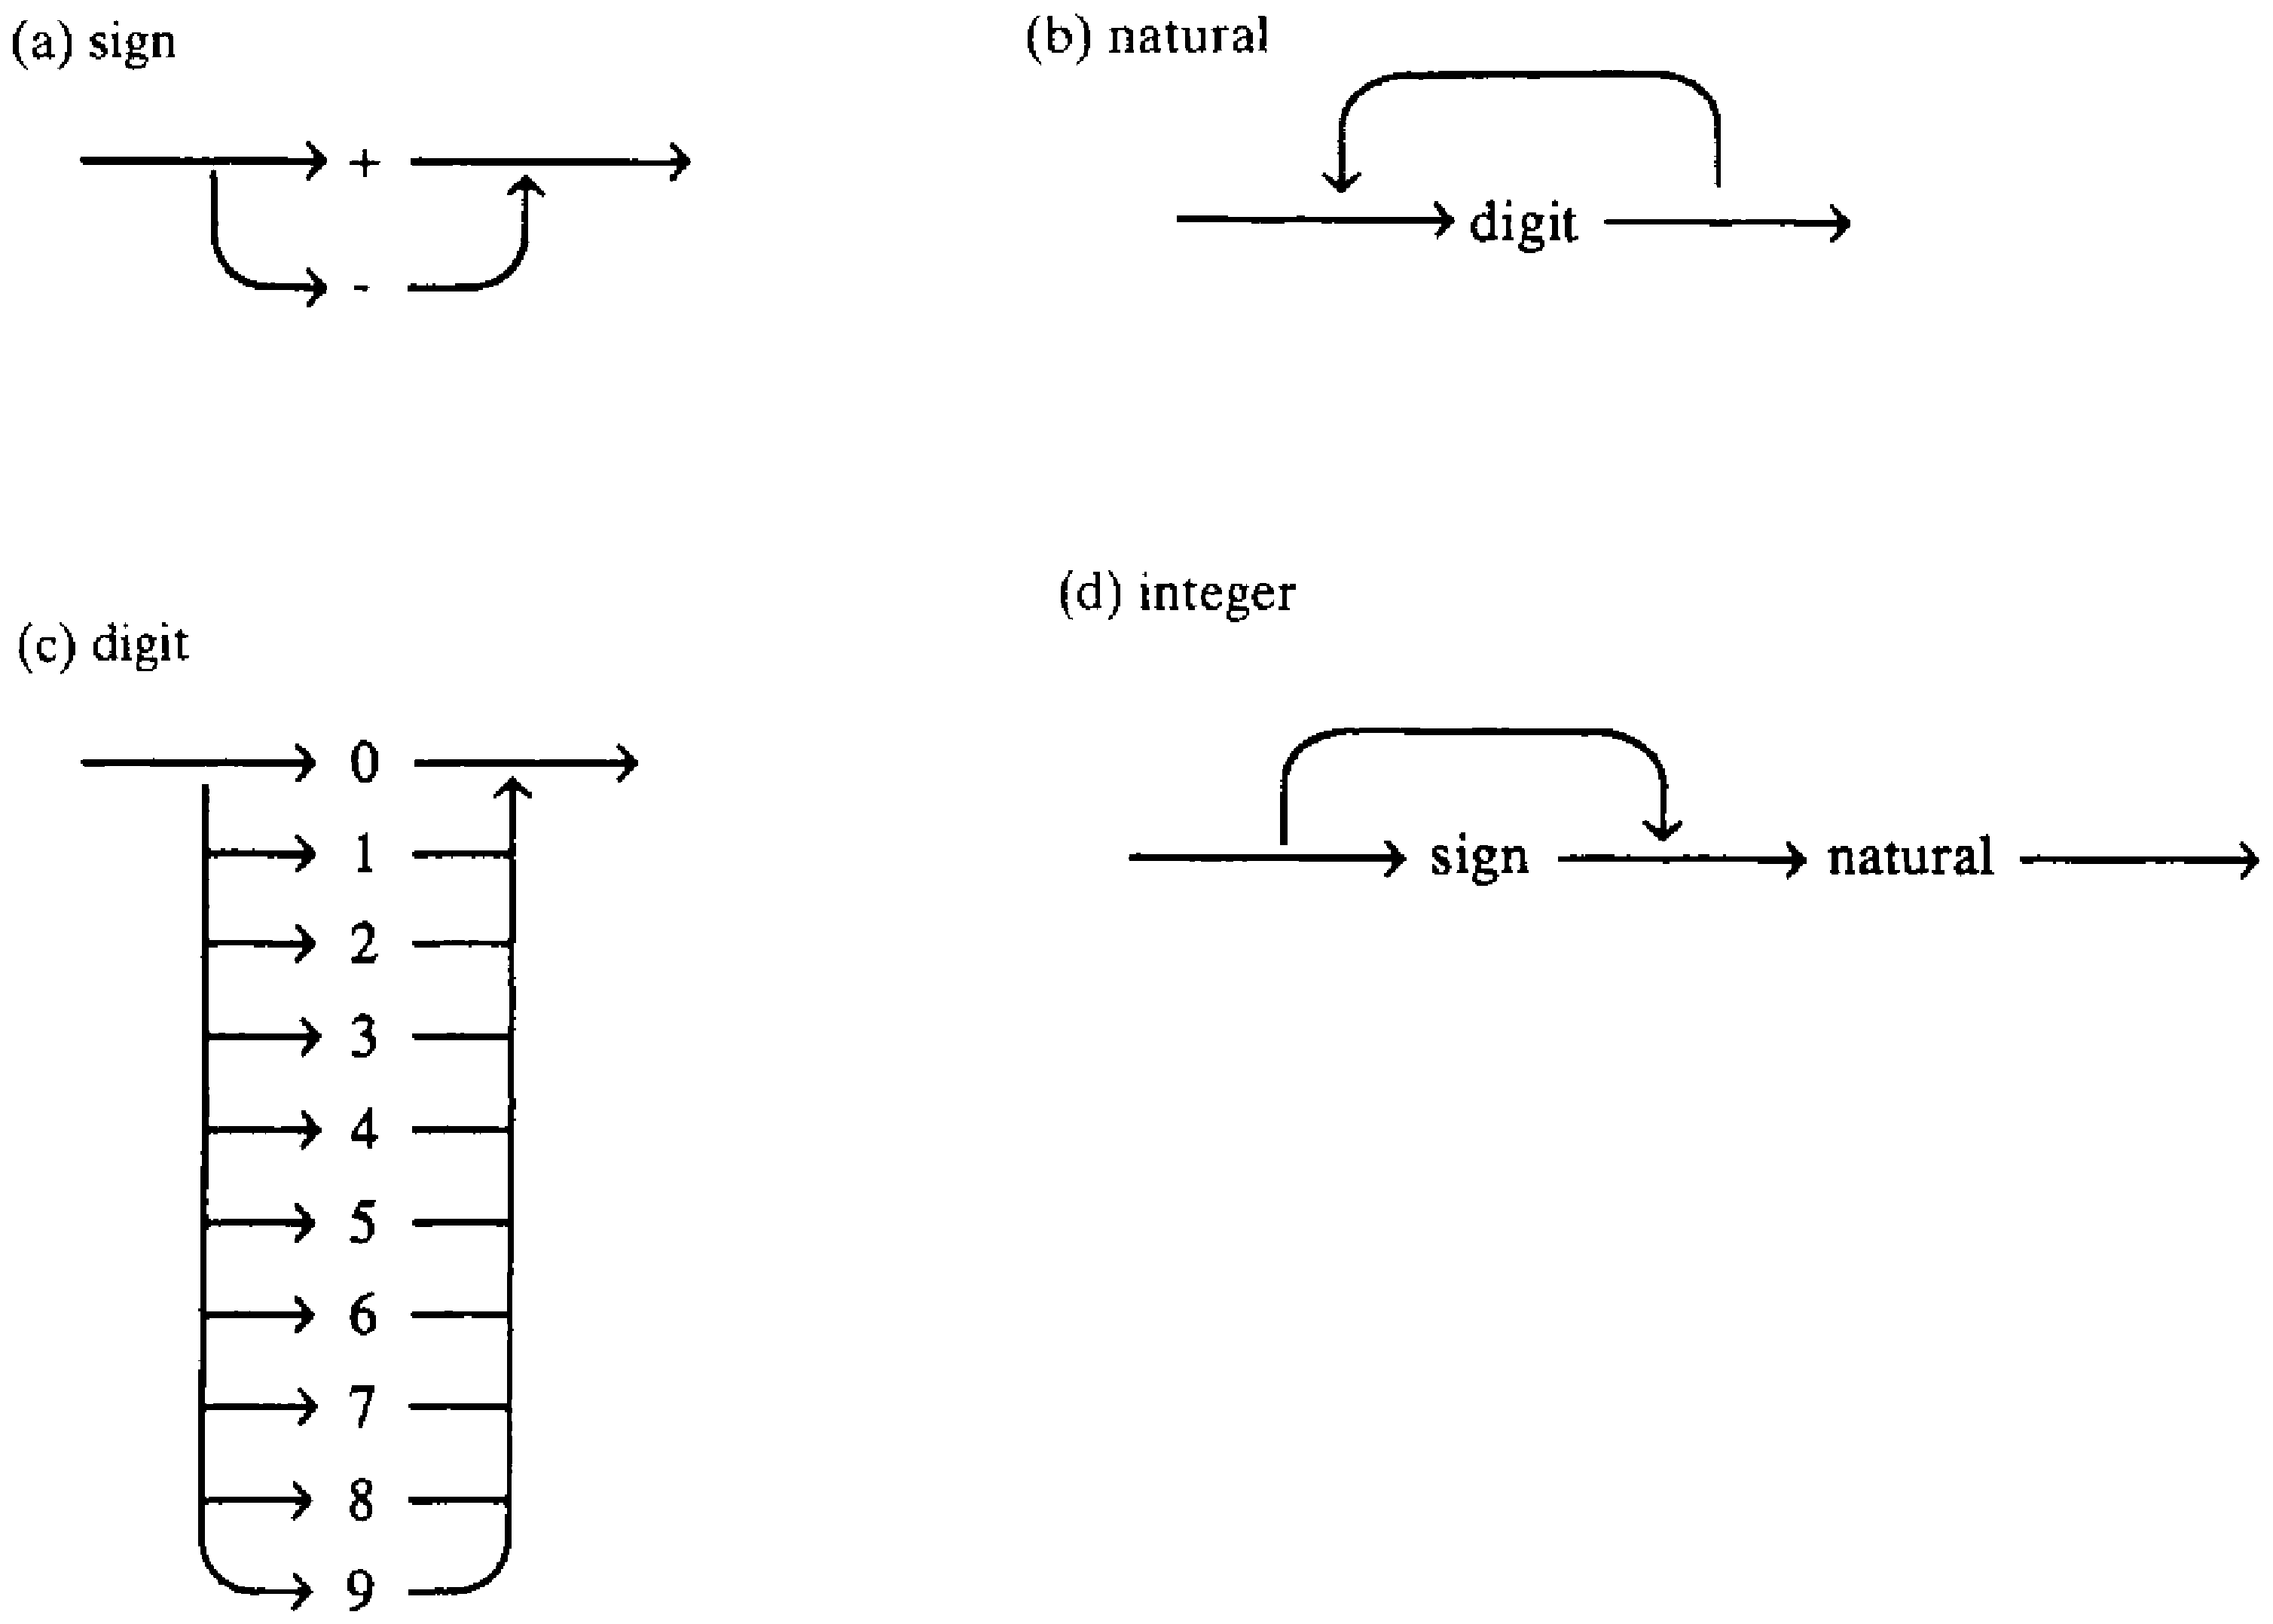
\epsfig{figure=ToFAfigures/fig0-6.eps,width=5.5in}}
%\centerline{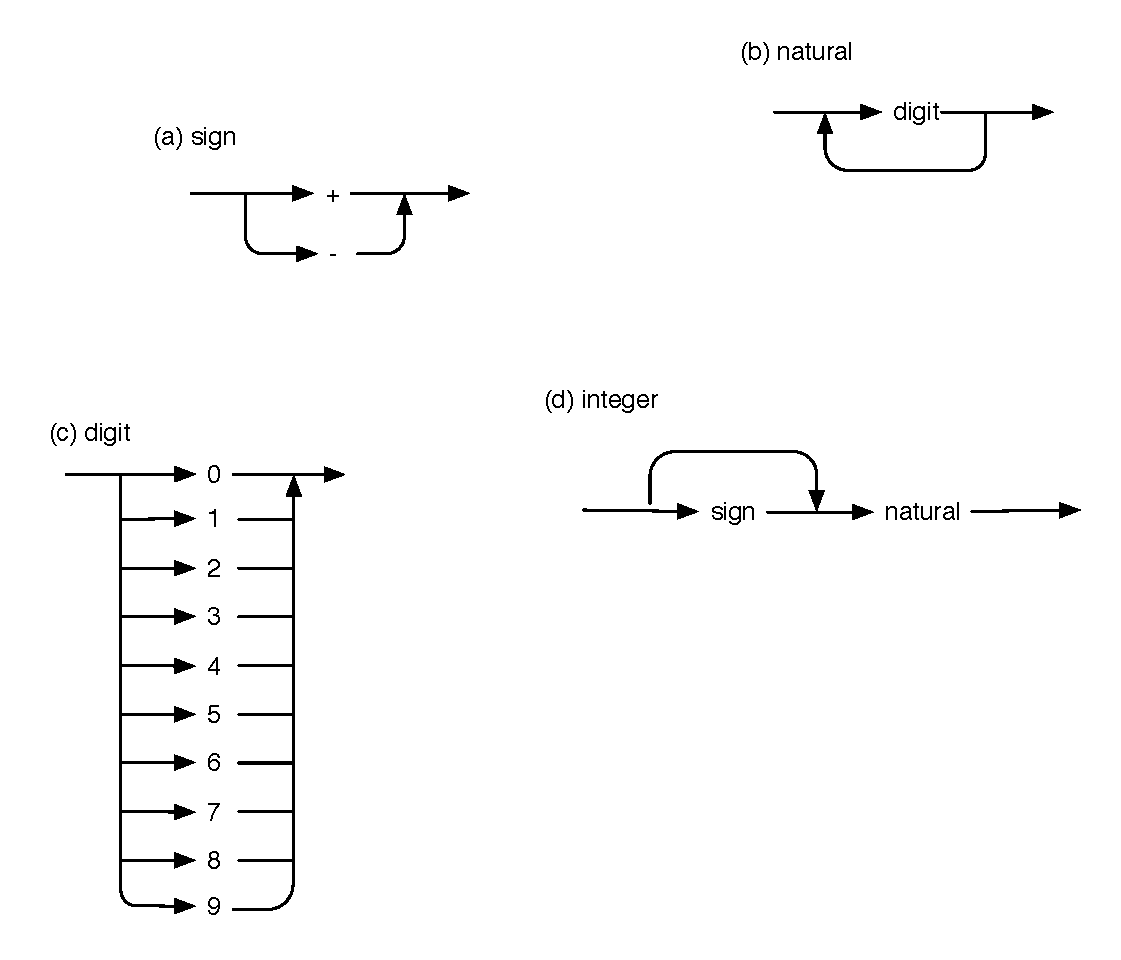
\epsfig{figure=Figures/fig-0-6.eps,width=\textwidth}}
%\centerline{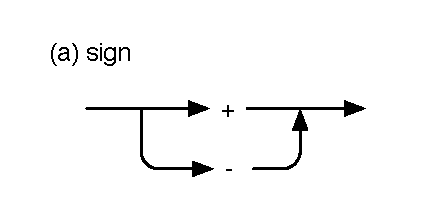
\epsfig{figure=Figures/fig-0-6-a.eps,width=0.25\textwidth}}
%\centerline{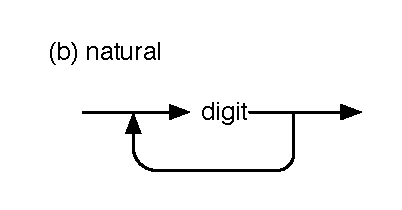
\epsfig{figure=Figures/fig-0-6-b.eps,width=0.25\textwidth}}
%\centerline{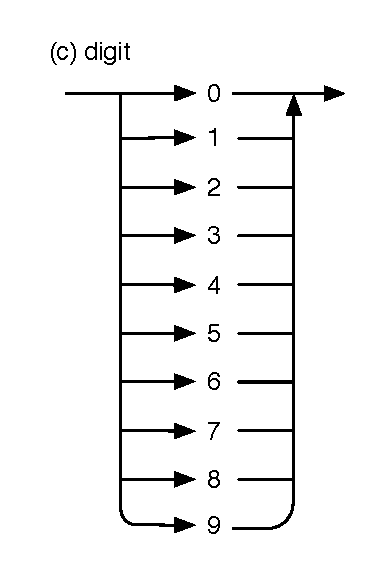
\epsfig{figure=Figures/fig-0-6-c.eps,width=0.25\textwidth}}
%\centerline{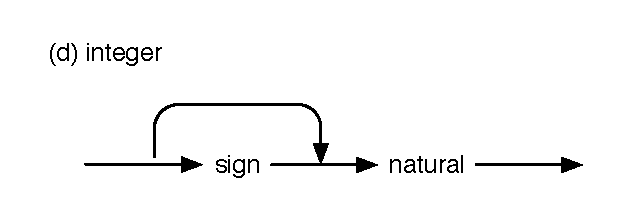
\epsfig{figure=Figures/fig-0-6-d.eps,width=0.25\textwidth}}
\caption{Syntax diagrams for the components of integer constants}\label{fig-0.6}
\end{figure}

\subsection*{Example 0.23}

The constraints for integer constants, which may begin with a sign and must
consist of one or more digits, are succinctly described by the following
\emph{productions} (replacement rules):
\begin{center}
\begin{tabular}{r@{ ::$=$ }l}
\<sign\> & $\pmb{+}|\pmb{-}$ \\
\<digit\> & $\pmb{0}|\pmb{1}|\pmb{2}|\pmb{3}|\pmb{4}|\pmb{5}|\pmb{6}|\pmb{7}|
	\pmb{8}|\pmb{9}$ \\
\<natural\> & \<digit\>$|$\<digit\>\<natural\>  \\
\<integer\> & \<natural\>$|$\<sign\>\<natural\> \\
\end{tabular}
\end{center}
The symbol $|$ represents ``or,'' and the rule
\[ \text{\<sign\> } ::= \pmb{+}|\pmb{-} \]
should be interpreted to mean that the token \<sign\> can be replaced by either
the symbol $\pmb{+}$ or the symbol $\pmb{-}$. A typical integer constant is
therefore $\pmb{+12}$, since it can be derived by applying the above rules in
the following fashion:
\begin{center}\begin{tabular}{r@{ $\rightarrow$ }l}
\<integer\> & \<sign\>\<natural\> \\
\<sign\>\<natural\> & $\pmb{+}$\<natural\> \\
$\pmb{+}$\<natural\> & $\pmb{+}$\<digit\>\<natural\> \\
$\pmb{+}$\<digit\>\<natural\> & $\pmb{+1}$\<natural\> \\
$\pmb{+1}$\<natural\> & $\pmb{+1}$\<digit\> \\
$\pmb{+1}$\<digit\> & $\pmb{+12}$
\end{tabular}\end{center}
Syntax diagrams for each of the four productions are shown in Figure \ref{fig-0.6}.
These can be combined to form a diagram that does not involve the intermediate
tokens \<sign\>, \<digit\>, and \<natural\> (see Figure \ref{fig-0.7}).

\begin{figure}[tb]
% Figure 0.7
%\centerline{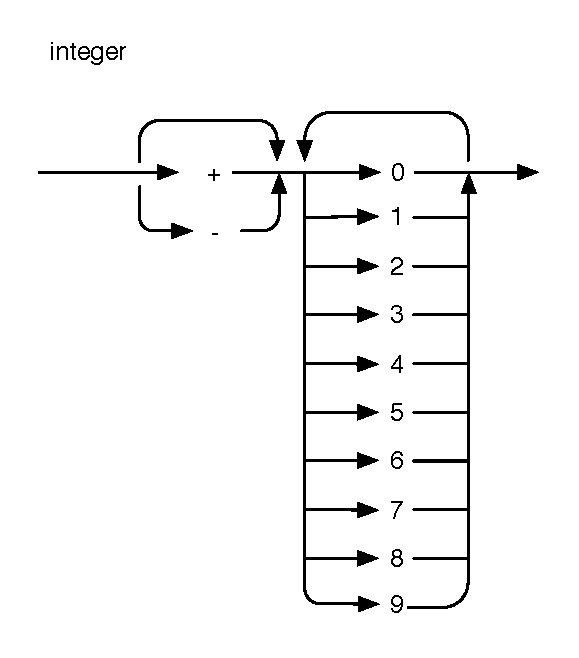
\epsfig{figure=Figures/fig-0-7.eps,width=\textwidth}}
\centerline{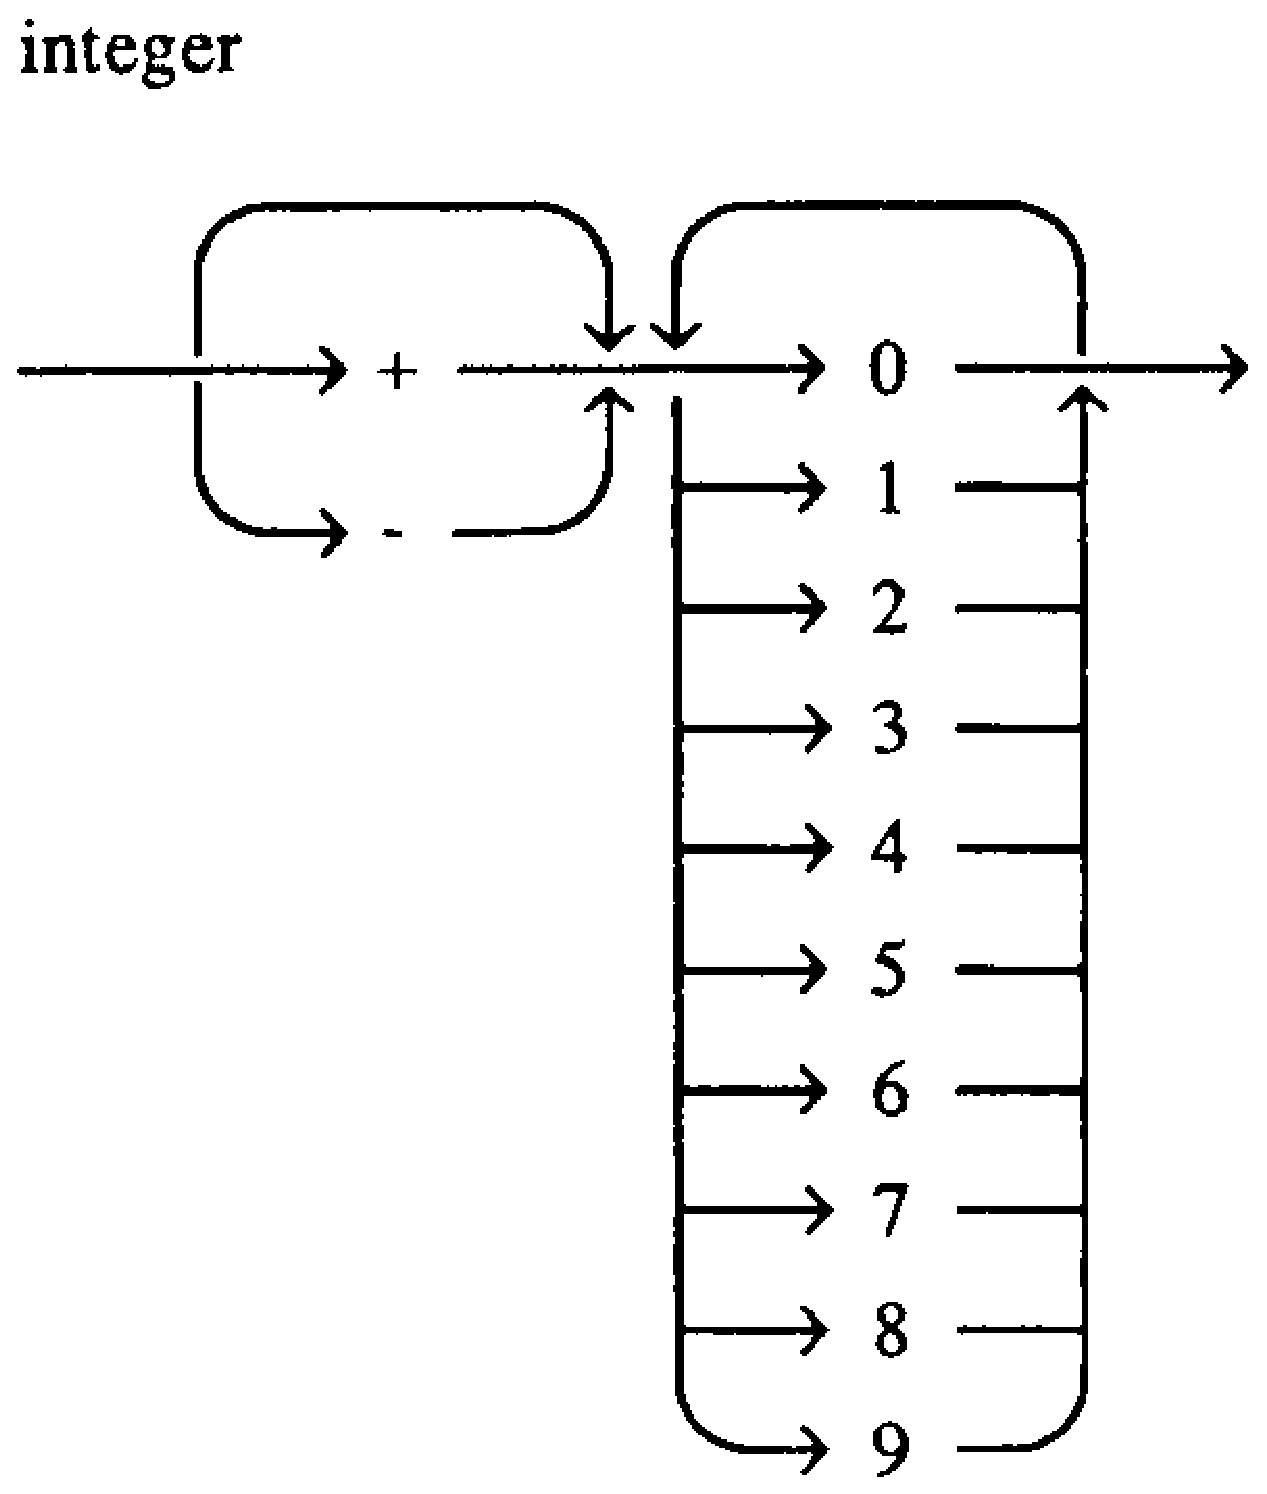
\epsfig{figure=ToFAfigures/fig0-7.eps,width=2.5in}}
\caption{A syntax diagram for integer constants}\label{fig-0.7}
\end{figure}

\section*{Exercises}\label{sec-0.exer}
\begin{enumerate}[{0.}1. ]
\item
Construct truth tables for:
\begin{enumerate}
\item
$\neg r \vee (\neg p \downarrow \neg q)$
\item
$(p \wedge \neg q) \vee \neg (p \uparrow  q)$
\end{enumerate}

\item
Draw circuit diagrams for:
\begin{enumerate}
\item $\neg (r \vee (\neg p \downarrow \neg q)) \uparrow (s \wedge p)$
\item $(p \wedge  \neg q) \vee \neg (p \uparrow q)$
\end{enumerate}

\item
Show that the sets $\{1, 2\} \times \{a, b\}$ 
and $\{a, b\} \times \{1, 2\}$ are not equal.

\item
Let $X =\{1, 2, 3, 4\}$.
\begin{enumerate}
\item
Determine the set of ordered pairs comprising the relation $<$.
\item
Determine the set of ordered pairs comprising the relation $=$.
\item
Since relations are sets of ordered pairs, it makes sense to union them
together.
Determine the set $= \cup <$.
\item
Determine the set of ordered pairs comprising the relation $\le$.
\end{enumerate}

\item
Let $n \in \NN$ be a natural number.
Show that congruence modulo $n$, $\equiv_n$, is an
equivalence relation.

\item
Let $X = \NN$.
Determine the equivalence classes for congruence modulo $0$.

\item
Let $X = \NN$. Determine the equivalence classes for congruence modulo $1$.

\item
Let $X = \RN$. Determine the equivalence classes for congruence modulo $1$.

\item
Let $R$ be an arbitrary equivalence relation in $X$.
Prove that the distinct equivalence classes of $R$ form a partition of $X$.

\item
Given a set $X$ and a partition $P = \{A_1,A_2, \ldots, A_n\}$ of $X$,
prove that $X$ equals the union of the sets in $P$.

\item
Given a set $X$ and a partition $P = \{A_1,A_2, \ldots, A_n\}$ of $X$, prove
that the relation $R(P)$ in $X$ induced by $P$ is an equivalence relation.

\item
Let $X = \{1, 2, 3, 4\}$.
\begin{enumerate}
\item
Give an example of a partition $P$ for which $R(P)$ is a function.
\item
Give an example of a partition $P$ for which $R(P)$ is not a function.
\end{enumerate}

\item
The following ``proof'' seems to indicate that a relation that is
symmetric and transitive must also be reflexive:

\begin{quote}
By symmetry, $x Ry \Rightarrow y Rx$. \\
Thus we have $(xRy \wedge yRx)$. \\
By transitivity, ($x Ry \wedge yRx) \Rightarrow x Rx$.\\
Hence $(\forall x)(x Rx)$.
\end{quote}

Find the flaw in this ``proof'' and give an example of a relation that is
symmetric and transitive but not reflexive.

\item
Let $R$ be an arbitrary equivalence relation in $X$. Prove that the equality
relation on $X$ refines $R$.

\item
Consider the ``function'' $t\!: \RN \rightarrow \RN$ defined by pairing $x$ with
the real number whose cosine is $x$.
\begin{enumerate}
\item
Show that $t$ is not well defined.
\item
Adjust the domain and range of $t$ to produce a valid function.
\end{enumerate}

\item
Consider the function $s'\!\!: \RN \rightarrow \RN$ defined by $s'(x) = x^2$ Show
that the converse of $s'$ is not a function.

\item
Let $\NNN$ be the set of nonnegative real numbers, and consider the function
$s$: $\NNN \rightarrow \NNN$ defined by $s(x)=x^2$. Show that $s^{-1}$ exists.

\item
Let $f$: $X\times Y$ be an arbitrary function. Prove that the converse of $f$ is
a function {\em iff} $f$ is a bijection.

\item
\begin{enumerate}
\item
Let $\sim$$A$ denote the complement of a set $A$. Prove that $\sim$$(\sim$$A) = A$.
\item
Let $\sim$$R$ denote the converse of a relation $R$. Prove that $\sim$$(\sim$$R) = R$
\end{enumerate}

\item
Let the functions $f$: $X \rightarrow Y$ and $g$: $Y \rightarrow Z$ be one to one.
Prove that $g \circ f$ is one to one.

\item
Let the functions $f$: $X \rightarrow Y$ and $g$: $Y \rightarrow Z$ be onto. Prove
that $g \circ f$ is onto.

\item
Define two functions for which $f\circ g = g\circ f$

\item
Define, if possible, a bijection between:
\begin{enumerate}
\item
$\NN$ and $\ZN$
\item
$\NN$ and $\NN \times \NN$
\item
$\NN$ and $\QN$
\item
$\NN$ and $\{a, b, c\}$
\end{enumerate}

\item
Use induction to prove that the sum of the cubes of the first $n$ positive
integers adds up to $\frac{n^2(n + 1)^2}{4}$

\item
Use induction to prove that the sum of the first $n$ positive integers is less
than $n^2$ (for $n > 1$).

\item
Use induction to prove that, for $n > 3$, $n! > n^2$.

\item
Use induction to prove that, for $n > 3, n! > 2^n$.

\item
Use induction to prove that $1^2 + 2^2 + \cdots + n^2 = n(n + 1)\frac{(2n + 1)}{6}$.

\item
Prove by induction that $X \cap (X_1 \cup X_2 \cup \cdots \cup X_n) =
(X \cap X_1) \cup (X \cap X_2) \cup \cdots \cup (X \cap X_n)$.

\item
Let $\sim A$ denote the complement of the set $A$. Prove by induction that
$\sim$$(X_1 \cup X_2 \cup \cdots \cup X_n) =
	(\sim$$X_1) \cap (\sim$$X_2) \cap \cdots \cap (\sim$$X_n)$.

\item
Use induction to prove that there are $2^n$ subsets of a set of size $n$; that
is, for any finite set $A$, $\|\wp(A)\| = 2^{\| A\|}$.

\item
The principle of mathematical induction is often stated in the following form,
which requires (apparently) stronger hypotheses to reach the desired conclusion:
Let $P(n)$ be a statement for each natural number $n \in \NN$. From the two
hypotheses
\begin{enumerate}[i.]
\item $P(0)$
\item $(\forall m \in \NN)(((\forall i \leq m)P(i)) \Rightarrow P(m + 1))$
\end{enumerate}
we can conclude $(\forall n \in \NN)P(n)$. Prove that the strong form of
induction is equivalent to the statement of induction given in the text.
\emph{Hint:} Consider the restatement of the hypothesis given in Example 0.22.

\item Determine what types of strings are defined by the following BNF:
\begin{center}\begin{tabular}{r@{ }l}
\<sign\> ::$=$ & $\pmb{+}|\pmb{-}$ \\
\<digit\> ::$=$ & $\pmb{0}|\pmb{1}|\pmb{2}|\pmb{3}|\pmb{4}|\pmb{5}|\pmb{6}|
	\pmb{7}|\pmb{8}|\pmb{9}$ \\
\<natural\> ::$=$ & \<digit\>$|$\<digit\>\<natural\> \\
\<integer\> ::$=$ & \<natural\>$|$\<sign\>\<natural\> \\
\<real constant\> ::$=$ & \<integer\> \\
& \<integer\>. \\
& \<integer\>.\<natural\> \\
& \<integer\>.\<natural\>{\bf E}\<integer\>
\end{tabular}\end{center}

\item A set $X$ is \emph{\Index{cofinite}} if the complement of $X$ (with respect to some generally
understood universal set) is finite. Let the universal set be $\ZN$. Give an
example of
\begin{enumerate}
\item A finite set
\item A cofinite set
\item A set that is neither finite nor cofinite
\end{enumerate}

\item Consider the equipotent relation, which relates sets to other sets.
\begin{enumerate}
\item Prove that this relation is reflexive.
\item Prove that this relation is symmetric.
\item Prove that this relation is transitive
\end{enumerate}

\item Define a function that will show that $\|\NN\| = \|\NN \times \NN\|$

\item Show that $\NN$ is equipotent to $\NN$.

\item Show that $\NN$ is equipotent to $\QN$.

\item Show that $\wp(\NN)$ is equipotent to $\{f$: $\NN\rightarrow\{$Yes, No$\}
\ |\ f$ is a function$\}$.

\item Show that $\wp(\NN)$ is equipotent to $\RN$.

\item Draw a circuit diagram that will implement the function $q$ given by the
truth table shown in Figure \ref{fig-0.8}.

\item \begin{enumerate}
\item Draw a circuit diagram that will implement the function $q_1$ given by the
truth table shown in Figure \ref{fig-0.9}.
\item Draw a circuit diagram that will implement the function $q_2$ given by the
truth table shown in Figure \ref{fig-0.9}.
\item Draw a circuit diagram that will implement the function $q_3$ given by the
truth table shown in Figure \ref{fig-0.9}.
\end{enumerate}
\end{enumerate}

% Figure 0.8
\begin{figure}[tb]
\begin{center}
\begin{tabular}{ccc|c}
$p_1$ & $p_2$ & $p_3$ & $q$\\
\hline
$\pmb{0}$ & $\pmb{0}$ & $\pmb{0}$ & $\pmb{0}$\\
$\pmb{0}$ & $\pmb{0}$ & $\pmb{1}$ & $\pmb{0}$\\
$\pmb{0}$ & $\pmb{1}$ & $\pmb{0}$ & $\pmb{1}$\\
$\pmb{0}$ & $\pmb{1}$ & $\pmb{1}$ & $\pmb{0}$\\
$\pmb{1}$ & $\pmb{0}$ & $\pmb{0}$ & $\pmb{1}$\\
$\pmb{1}$ & $\pmb{0}$ & $\pmb{1}$ & $\pmb{0}$\\
$\pmb{1}$ & $\pmb{1}$ & $\pmb{0}$ & $\pmb{0}$\\
$\pmb{1}$ & $\pmb{1}$ & $\pmb{1}$ & $\pmb{1}$
\end{tabular}
\end{center}
\caption{The truth table for Exercise 0.41}\label{fig-0.8}
\end{figure}

% Figure 0.9
\begin{figure}[tb]
\begin{center}
\begin{tabular}{cccc|ccc}
$p_1$ & $p_2$ & $p_3$ & $p_4$ & $q_1$ & $q_2$ & $q_3$\\
\hline
$\pmb{0}$ & $\pmb{0}$ & $\pmb{0}$ & $\pmb{0}$ & $\pmb{1}$ & $\pmb{1}$ & $\pmb{1}$\\
$\pmb{0}$ & $\pmb{0}$ & $\pmb{0}$ & $\pmb{1}$ & $\pmb{0}$ & $\pmb{1}$ & $\pmb{0}$\\
$\pmb{0}$ & $\pmb{0}$ & $\pmb{1}$ & $\pmb{0}$ & $\pmb{1}$ & $\pmb{0}$ & $\pmb{0}$\\
$\pmb{0}$ & $\pmb{0}$ & $\pmb{1}$ & $\pmb{1}$ & $\pmb{1}$ & $\pmb{1}$ & $\pmb{0}$\\
$\pmb{0}$ & $\pmb{1}$ & $\pmb{0}$ & $\pmb{0}$ & $\pmb{0}$ & $\pmb{1}$ & $\pmb{1}$\\
$\pmb{0}$ & $\pmb{1}$ & $\pmb{0}$ & $\pmb{1}$ & $\pmb{1}$ & $\pmb{0}$ & $\pmb{0}$\\
$\pmb{0}$ & $\pmb{1}$ & $\pmb{1}$ & $\pmb{0}$ & $\pmb{1}$ & $\pmb{1}$ & $\pmb{0}$\\
$\pmb{0}$ & $\pmb{1}$ & $\pmb{1}$ & $\pmb{1}$ & $\pmb{0}$ & $\pmb{0}$ & $\pmb{0}$\\
$\pmb{1}$ & $\pmb{0}$ & $\pmb{0}$ & $\pmb{0}$ & $\pmb{1}$ & $\pmb{0}$ & $\pmb{1}$\\
$\pmb{1}$ & $\pmb{0}$ & $\pmb{0}$ & $\pmb{1}$ & $\pmb{1}$ & $\pmb{0}$ & $\pmb{0}$\\
$\pmb{1}$ & $\pmb{0}$ & $\pmb{1}$ & $\pmb{0}$ & $\pmb{0}$ & $\pmb{1}$ & $\pmb{0}$\\
$\pmb{1}$ & $\pmb{0}$ & $\pmb{1}$ & $\pmb{1}$ & $\pmb{0}$ & $\pmb{0}$ & $\pmb{0}$\\
$\pmb{1}$ & $\pmb{1}$ & $\pmb{0}$ & $\pmb{0}$ & $\pmb{1}$ & $\pmb{1}$ & $\pmb{1}$\\
$\pmb{1}$ & $\pmb{1}$ & $\pmb{0}$ & $\pmb{1}$ & $\pmb{0}$ & $\pmb{1}$ & $\pmb{0}$\\
$\pmb{1}$ & $\pmb{1}$ & $\pmb{1}$ & $\pmb{0}$ & $\pmb{0}$ & $\pmb{1}$ & $\pmb{1}$\\
$\pmb{1}$ & $\pmb{1}$ & $\pmb{1}$ & $\pmb{1}$ & $\pmb{0}$ & $\pmb{0}$ & $\pmb{0}$
\end{tabular}
\end{center}
\caption{The truth table for Exercise 0.42}\label{fig-0.9}
\end{figure}
